\section{Introduction}
\label{sec:classif:intro}

The Brazilian science system exists primarily within graduate programs (PPG), composed of master's and doctoral levels. This design was not an accident, but a consequence of a science system that did not develop spontaneously; it was the object of public policy that prioritized the link between research and education. Most of that effort took place from the 1950s, initially by shaping the system and then towards its expansion \autocite{Balbachevsky.2010, Brasil.2020}. One of the key strategies adopted was implementing a scholarship system to allow Brazilians to pursue degrees either abroad – aiming to build a critical mass to materialize the country's graduate education – or in the growing number of resulting master's and doctoral courses in Brazil \autocite{CNPG.1974, Gouvea.2012}.

In the early 1970s, the number of scholarship holders from the leading agency in charge of funding the research and graduate system in the country, CAPES, was significantly small. The agency's grant report from 1971 revealed that only 1831 scholarships were awarded for graduate students in the country, and an additional 134 were granted to study abroad. Because of the manageable numbers, scholarships were handled mainly by a deliberative council that would analyse candidates in the face of the available funding. According to Darcy Closs, CAPES' executive director from 1974 to 1979, this process was particularly challenging, as many national figures would pressure the council into awarding grants to proteges \autocite{Castro.1983, Cordova.2001, Ferreira.2002}. 

Aiming to avoid lobbying, CAPES sought inspiration from the peer review experience of accreditation agencies in the USA. The first effort in Brazil, still in 1974, consisted of the installation of a single peer review committee with a small group of experts from broad areas such as engineering and social sciences. Academic merit would guide decisions on scholarship distribution and the list of awardees would be submitted to the minister of education for endorsement. The task at hand was beyond the certification of the results, as the real challenge was neutralizing the complaints of influential people who had their requests denied. Reports on the initiative of the advisory committee acknowledge that positive results were only possible due to the performance of the minister in protecting the newly established merit system \autocite{Ferreira.2002}.

However, the single committee would not be able to keep up with the number of scholarships granted every year, which grew over 400\% in under a decade \autocite{Castro.1983}. Therefore, two significant changes were implemented: (i) Evaluation evolved to an institutional model, where CAPES would assess graduate programs instead of individual candidates, granting a quota of scholarships to the programs based on performance. Then, the PPG would distribute the scholarships based on internal criteria; (ii) The original advisory committee was transformed into a series of disciplinary committees, which multiplied according to the growth in graduate programs and consequential increase in demand \autocite{Cordova.2001, Ferreira.2002}.

According to the most recent official reports, in early 2021, there were 4459 graduate programs active in Brazil, and CAPES granted around 95.000 scholarships for master's and doctoral courses in the country and 4494 for study and research abroad. The distribution of these scholarships is still heavily based on the evaluation performance of the graduate programs, with a system organized around 49 evaluation areas, which developed from the disciplinary peer review committees \autocite{CAPES.2020tb, CAPES.2021g}.

This study looks at the current evaluation areas and analyses whether a reorganization may be necessary. For that, we consider three different perspectives: (i) the dynamics of the expansion of evaluation areas and observed inconsistencies in how they are organized; (ii) an international comparison of classification systems of research and education; (iii) a recommendation from a special committee in charge of monitoring the Brazilian National Plan for Research and Graduate Education (PNPG)\footnote{See \textcite{Brasil.2020} for further discussion on the National Plans for Graduate Education.}. Finally, after identifying weaknesses in the structuring of the Brazilian evaluation areas, the study advances to propose a bibliometric approach to rethink such areas and the distribution of graduate programs within them.

\section{Evaluation areas and their roles}
\label{sec:classif:eval_areas}

Evaluation areas are a core component of the established evaluation system in Brazil. Each area counts with its peer review committee, coordinated by representatives appointed by graduate programs in each discipline and nominated by CAPES for a four-year term. The coordinator's work is supported by two deputies, one for academic and the other for professional programs. Although broader regulations guide national evaluation, each area has some freedom to determine specific criteria and indicators in its analyses \autocite{141/2016}. For instance, as described in a previous study, areas can choose which types of technical and technological products should be recognized as suitable research outputs, being valued by the committees in the evaluation process \autocite{Brasil.2021a}.

The configuration in 49 areas also has a pivotal role in the organization of the science system. Accreditation of new graduate programs is mandatory in the country. Once a proposal is approved, the new PPG becomes part of the corresponding area, subject to their specific evaluation criteria. Additionally, every four years, accreditation must be renewed in a national evaluation that is comparative within each area. PPG are graded on a scale of 1 through 7 based on how they fare against the overall performance of the other programs in the same areas \autocite{Brasil.2022e, 122/2021}. The evident relevance of the evaluation areas is established even in related legislation, where they are given the responsibility to guide CAPES' programs and courses of action \autocite{141/2016}. 

\Cref{tab:classif:areas} shows CAPES evaluation areas, with unique identifiers in parentheses, aggregated into the nine broad areas and three upper groups adopted by the agency \autocite{CAPES.2020tb}.

{\footnotesize \renewcommand{\arraystretch}{1.3} \linespread{0.8}
\begin{xltabular}{\linewidth}{@{}L{2cm}L{3cm}X@{}}
\caption{CAPES evaluation areas according to their respective broad areas and upper groups}\label{tab:classif:areas}\\ 

\toprule
\textbf{Upper Group} & \textbf{Broad area} & \textbf{Evaluation area}  \\\midrule

\endfirsthead

\multicolumn{3}{r@{}}{\Cref*{tab:classif:areas} Continued}\\ 
\toprule
\textbf{Upper Group} & \textbf{Broad area} & \textbf{Evaluation area}  \\\midrule

\endhead

\bottomrule
\multicolumn{3}{l@{}}{Continue\ldots}\\ 
\endfoot

\bottomrule
\multicolumn{3}{c@{}}{Source: \textcite{CAPES.2020tb}}
\endlastfoot

\textbf{Exact Sciences} & Engineering & Engineering I (10), 
Engineering II (12), 
Engineering III (13), 
Engineering IV (14) \\
 & Exact and Earth Sciences & Astronomy and physics (03), 
Chemistry (04), 
Computer science (02), 
Earth sciences (05), 
Mathematics and statistics (01) \\
 & Multidisciplinary & Biotechnology (48), 
Environmental sciences (49), 
Interdisciplinary (45), 
Materials science (47), 
Teaching and learning (46) \\ \midrule
\textbf{Humanities} & Applied Social Sciences & Architecture, interior and industrial design (29), 
Business and administration, accounting and tourism (27), 
Economics (28), 
Journalism and information (31), 
Law (26), 
Social work (32), 
Town planning and demography (30) \\
 & Humanities & Anthropology and archaeology (35), 
Education (38), 
Geography (36), 
History (40), 
Philosophy and ethics (33), 
Political Science and international relations (39), 
Psychology (37), 
Religion and theology (44), 
Sociology (34) \\
 & Linguistics, Literature and Arts & Arts (11), 
Literature and linguistics (41) \\ \midrule
\textbf{Life Sciences} & Agricultural Sciences & Agricultural sciences (42), 
Food science and technology (25), 
Veterinary medicine (24), 
Zootechnics and fisheries (23) \\
 & Biological Sciences & Biodiversity (07), 
Biological Sciences I (06), 
Biological Sciences II (08), 
Biological Sciences III (09) \\
 & Health Sciences & Dental studies (18), 
Medicine I (15), 
Medicine II (16), 
Medicine III (17), 
Nursing (20), 
Nutritional science (50), 
Pharmacy (19), 
Physical education, therapy and rehabilitation (21), 
Public health (22) \\

\end{xltabular}
}

Although the names of some evaluation areas shown in \Cref{tab:classif:areas} are very descriptive, such as ‘Environmental sciences’ or ‘Computer science’, others are more difficult to understand unless subareas or specialties are considered. For instance, \textcite{CAPES.2020tb} shows that electrical and biomedical engineering are subareas included in ‘Engineering IV’, and that ‘Medicine I’ aggregates specialties such as oncology and cardiology. 

In addition to existing cryptical names, some evaluation areas combine broader sets of disciplines with different levels of affinity for their objects, cognitive methods, and instrumental resources. A significant example is in ‘anthropology and archaeology’, which combines the disciplines in a single evaluation area, under the broad area of 'humanities'. The American Academy of Arts and Sciences, for instance, considers archaeology to be part of the humanities, and anthropology to be a social science, despite recognising its humanistic perspective \autocite{AAAS.2022}. 

The evaluation area system designed by CAPES evolved according to the dynamics of the agency and the expansion of the country's research and graduate education system. Over time, new areas have been created and others have been combined or restructured in ways that led to some mismatch with other classification systems, such as the OECD Fields of Research and Development (FORD) and UNESCO’s International Standard Classification of Education (ISCED). Some of these inconsistencies are visible in Figures 1 and 2, where CAPES’ broad areas were matched against FORD’s and ISCED’s broad classifications. For that, multilevel analysis was conducted based on areas, subareas, and specialties for the three systems \autocite{OECD.2015fr, UNESCO.2015, CAPES.2020tb}.

\begin{figure}[ht]
\vspace{8pt}
    \centering
    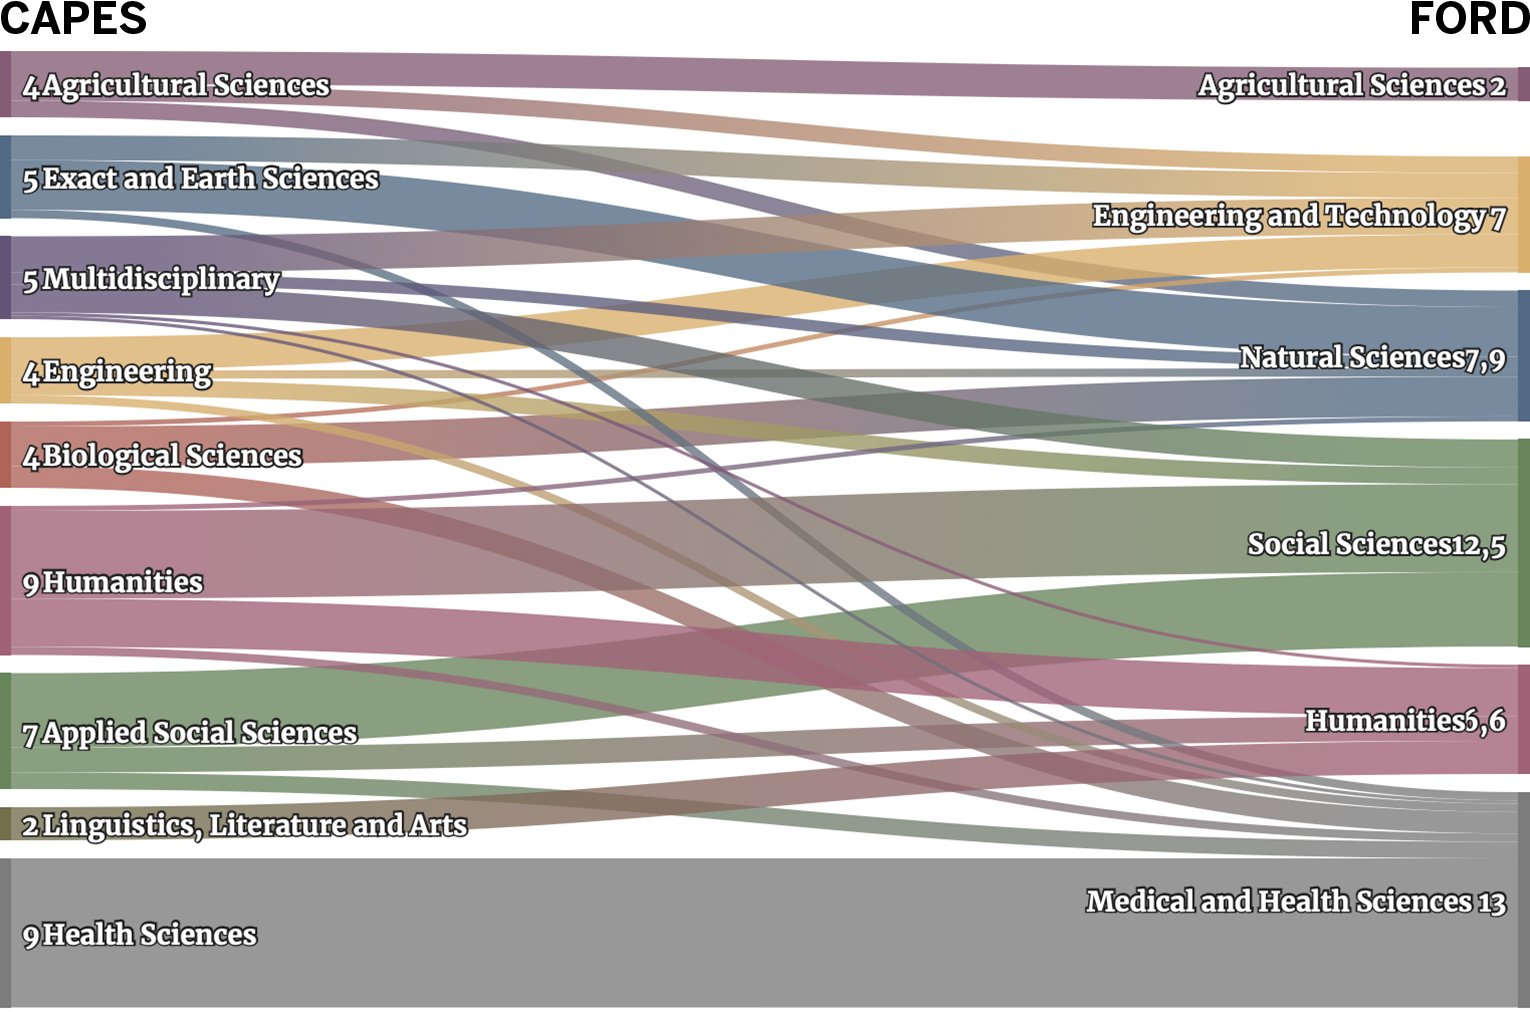
\includegraphics[width=1\textwidth]{images/chapter_classific/capes_oecd.png}
    \caption{CAPES broad area relations with FORD’s broad classification.}
    \label{fig:classif:capes_ford}
\end{figure}

\Cref{fig:classif:capes_ford} shows the nine broad areas in the CAPES classification system on the left, with numbers representing how many evaluation areas are included. Fractional numbers can be seen on the FORD part of the Sankey chart, as areas or subareas from the Brazilian system may be split into different groups as they were defined by \textcite{OECD.2015fr}. For the broad group of Biological Sciences, for example, some subareas of ‘Biological sciences III’ fit within ‘Medical and Health Sciences’ (e.g., immunology and parasitology) and others belong to ‘Engineering and Technology’ in the FORD schema (e.g., cell \& tissue engineering).

Another distinction between the two systems connected in Figure 1 relates to the social sciences and humanities, as some inconsistencies can be seen in the distribution of the groups across the distinct classifications. For instance, more than half of what CAPES considers to be part of the humanities is classified as social sciences by FORD (e.g., political science and psychology). One could argue that the Brazilian system is designed with graduate education in mind, which could lead to the observed conflicts. However, such mismatches in SSH are also visible in \Cref{fig:classif:capes_isced}, where CAPES broad areas are connected to ISCED’s classification.

\begin{figure}[ht]
\vspace{8pt}
    \centering
    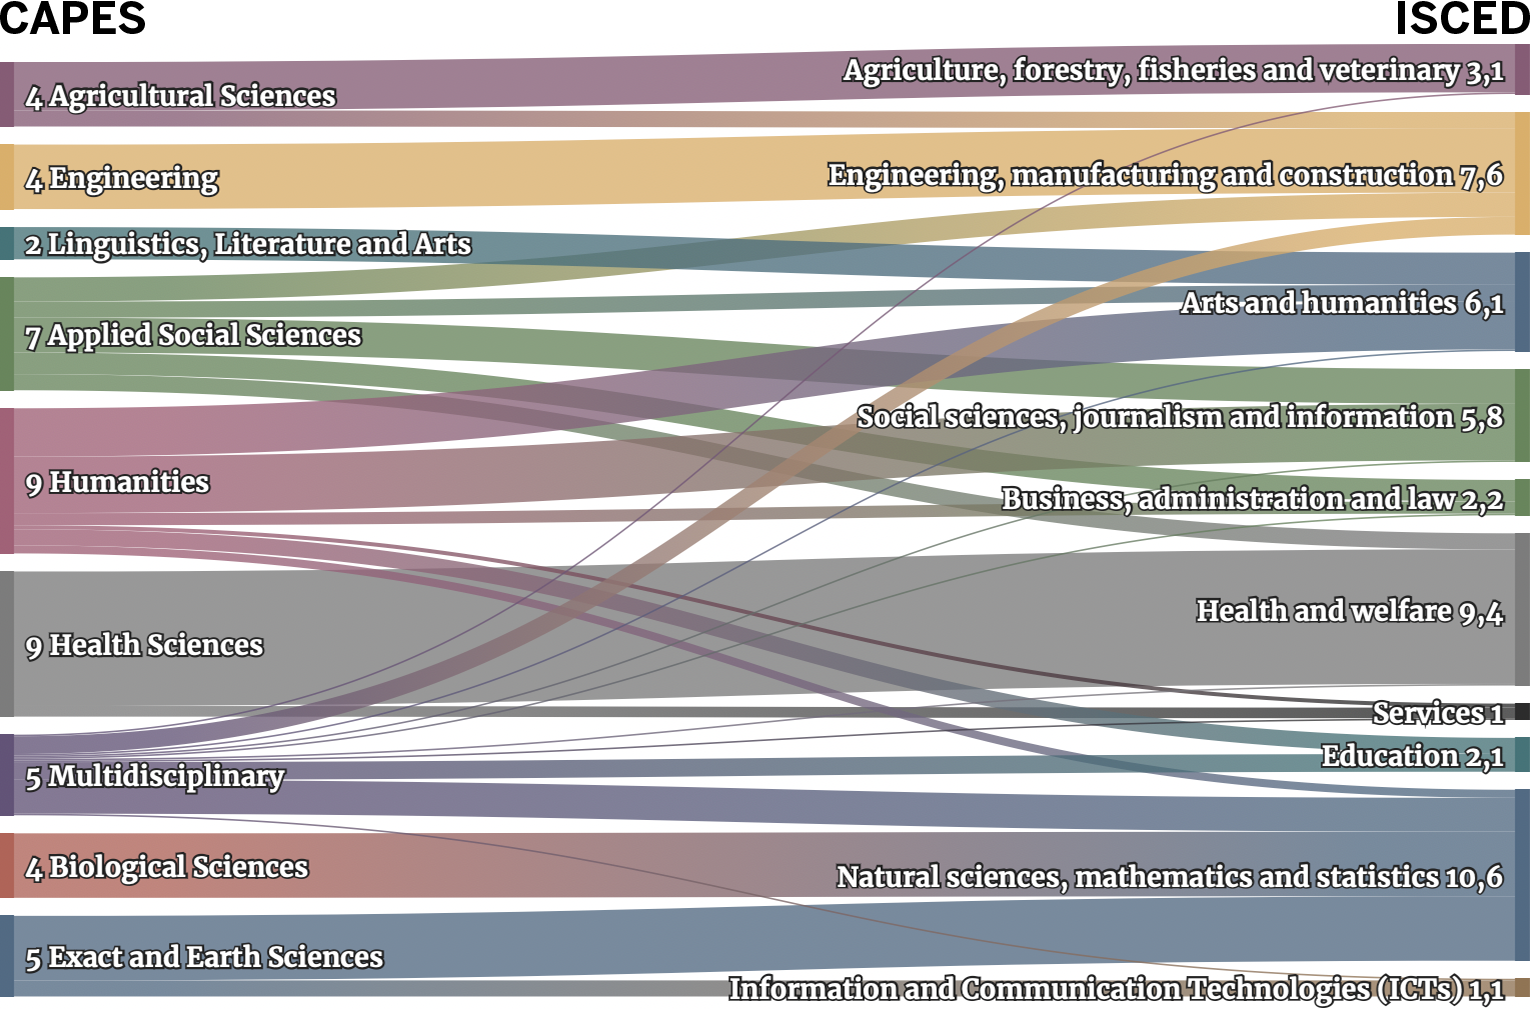
\includegraphics[width=1\textwidth]{images/chapter_classific/capes_isced.png}
    \caption{CAPES broad area relations with ISCED’s broad classification.}
    \label{fig:classif:capes_isced}
\end{figure}
 
The ISCED groups are significantly different from the FORD ones, especially due to broad classifications such as ‘Services’, ‘Education’, and ‘ICTs’. Once again, the connections between SSH disciplines are very inconsistent. Also, CAPES multidisciplinary broad area has a small connection to nearly all the ISCED groups, as the system counts with a specific code in each group to include interdisciplinary programs and qualifications. Therefore, many of the different graduate programs within CAPES ‘Interdisciplinary’ evaluation area find a specific home within the ISCED classification.

\section{Rethinking the Brazilian classification}
\label{sec:classif:rethinking}

The differences between the main classification system adopted in Brazil and international alternatives such as FORD and ISCED are a problem for the country to conduct comparative studies on funding allocation, research dynamics in countries and disciplines, scientometrics, etc. Although matching classification systems at their most granular levels – like what has been done for this paper – can help conduct some of the types of studies mentioned, the time-consuming activity is unlikely to be replicated widely and consistently. A solution would be to review the Brazilian classification for better international equivalence, and the same has been suggested by the special committee in charge of monitoring the Brazilian National Plan for Research and Graduate Education (PNPG). 

Since the 1970s, Brazil has issued periodic PNPG to help guide evaluation and science funding policies in the country \autocite{Brasil.2020}. The most recent plan covered the period 2011-2020, with execution and results being monitored by a special committee. At the end of their term, the group prepared a report with many recommendations, including the need to rethink the current classification system, as the 49 areas do not reflect the modern panorama of science \autocite{CEPNPG.2020}. Although the committee’s recommendation for change is aligned with the findings of this study, there is a significant disagreement on the methods.

The \textcite{CEPNPG.2020} report suggests a substantial reduction in the number of evaluation areas, using the nine broad areas as a reference. However, we have seen significant discrepancies between CAPES broad areas and those of international classifications. Furthermore, merging areas may represent a setback to a crucial achievement for research evaluation. After decades of area expansion, peer review committees achieved a level of freedom to customize evaluation criteria to suit their practices and value their principles. Moreover, the comparative perspective of the evaluation system has value when similar PPG exist within each area but can be damaging in heterogeneous environments. Perhaps, the most adequate approach is not aiming for numbers, but for an adequate distribution of research that can be suitable for national evaluation and funding purposes, as well as international comparisons.

A possible method for reviewing the classification system may be supported by bibliometrics. To demonstrate one possibility, microdata of the 2017-2018  papers from the three biological science areas (BioSci) have been collected from CAPES Open Data System \autocite{CAPES.2021d}. Information such as DOI, ISSN, authorship, volume, page numbers, etc. was used to match the publications to Web of Science.

Departing from the 15.370 documents matched to WoS, a term map of BioSci papers was produced using VOSviewer software \autocite{Eck.2009}. For that, the title and abstracts of the articles were collected from WoS \autocite{Clarivate.2022}. Binary counting was used to extract over 280 thousand noun phrases from the corpus, of which 8161 appeared in at least ten documents. A relevance score was calculated for each of these terms, with a threshold of 60\%, and the resulting 4897 terms were used to produce the map seen in \Cref{fig:classif:vosviewer_cb}.

\begin{figure}[ht]
\vspace{8pt}
    \centering
    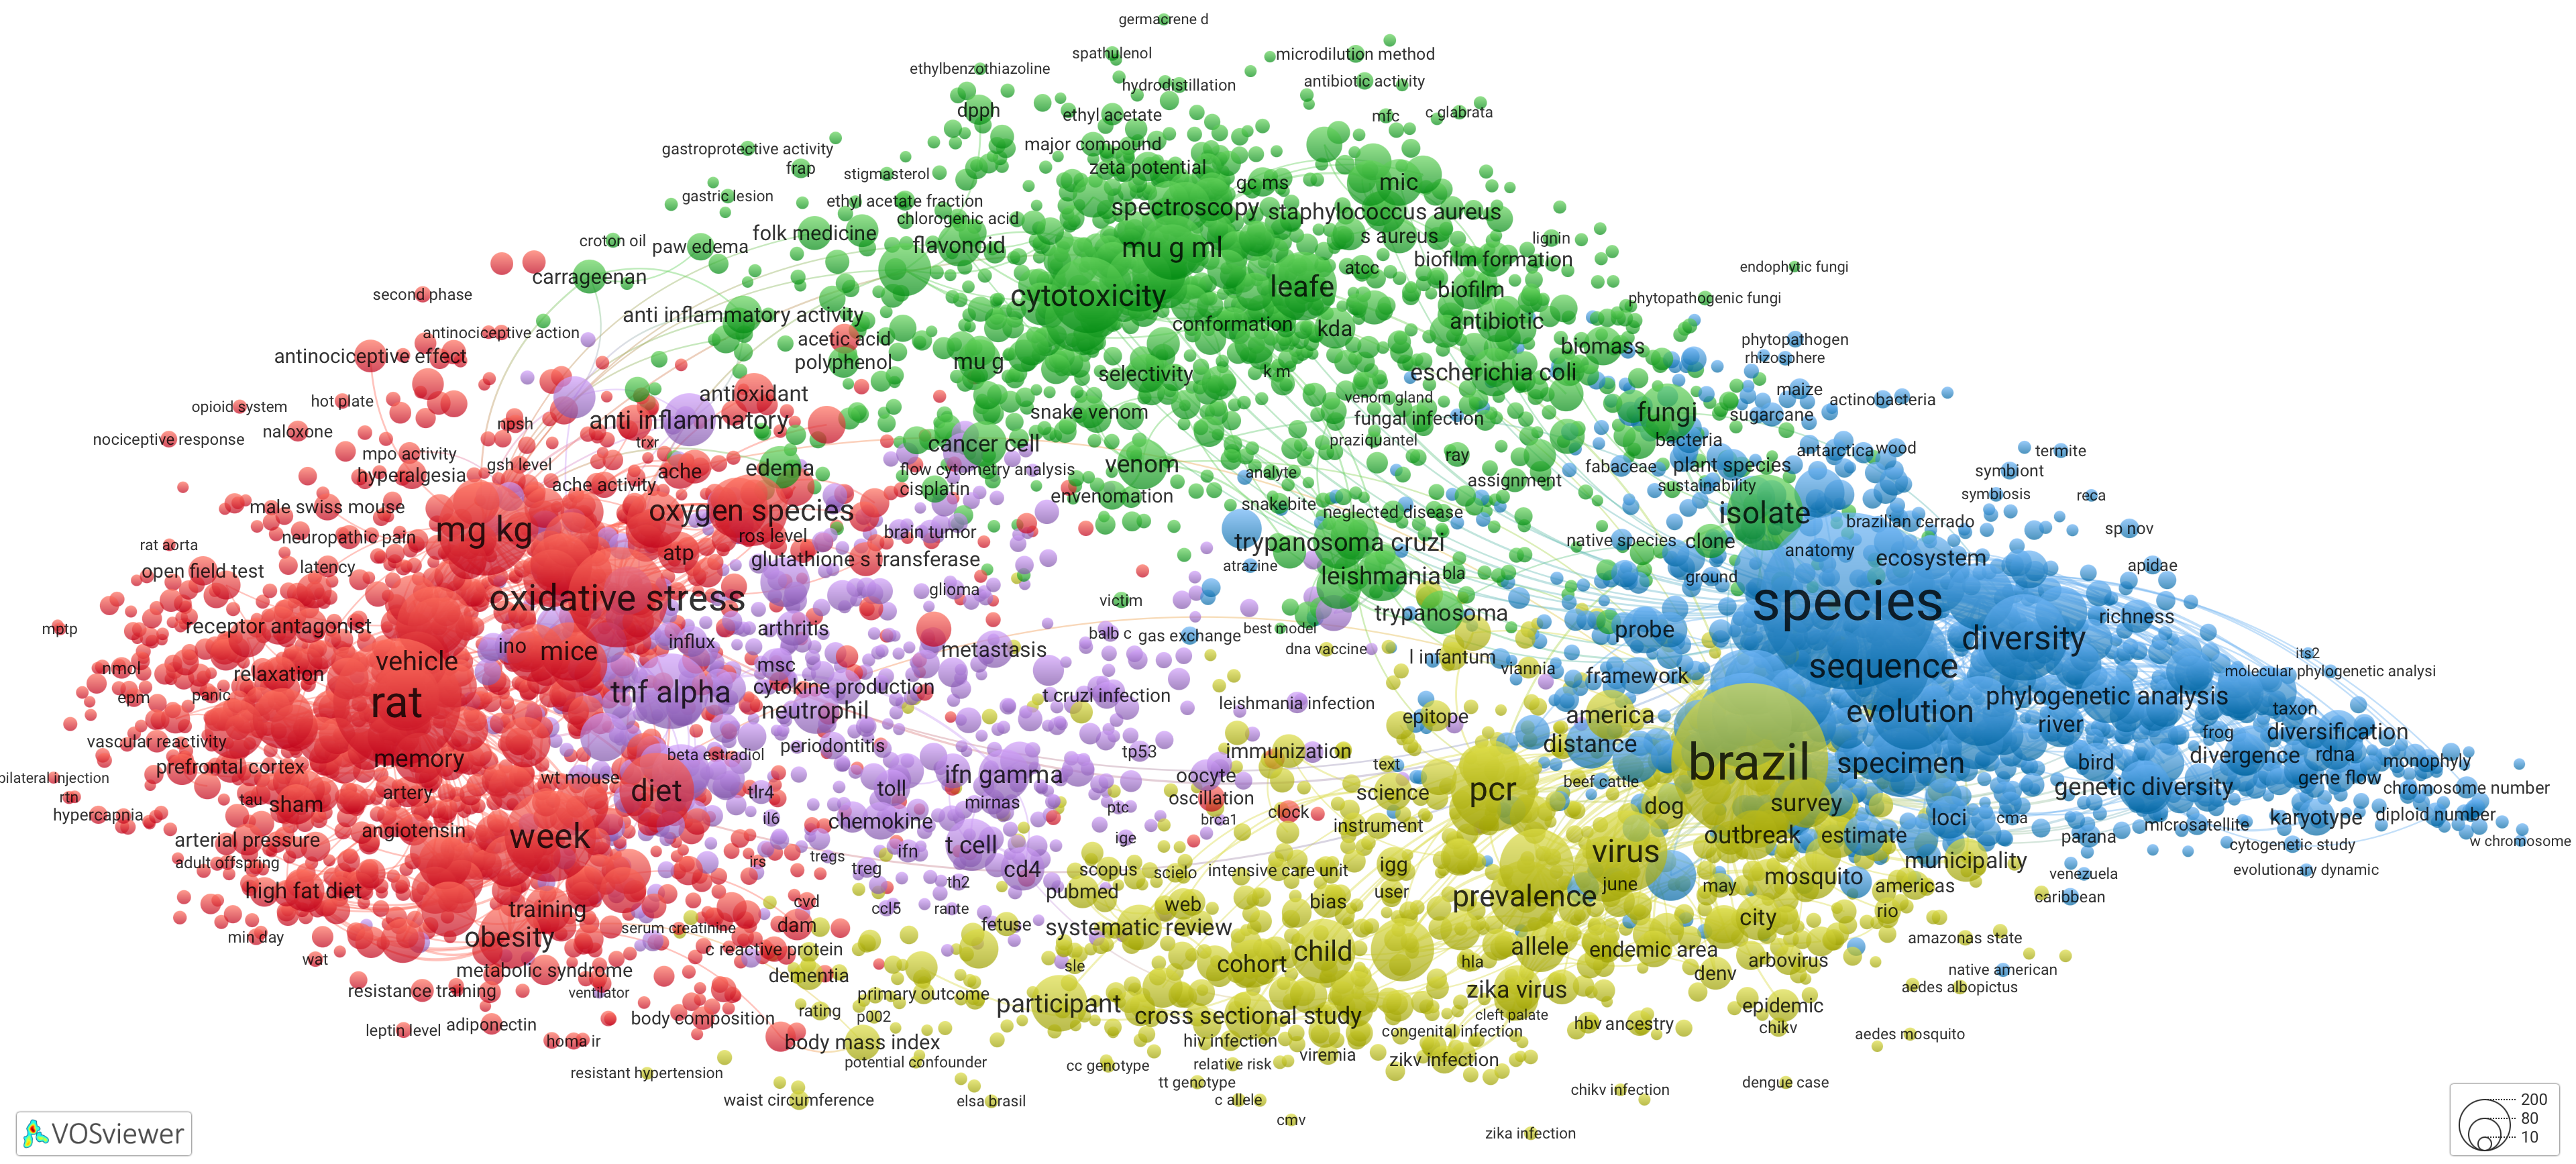
\includegraphics[width=1\textwidth]{images/chapter_classific/VOSviewer-CB-clusters.png}
    \caption{Term map of papers from the Biological Sciences evaluation areas (2017-2018).}
    \label{fig:classif:vosviewer_cb}
\end{figure}
 
In \Cref{fig:classif:vosviewer_cb}, the size of each circle represents the number of documents in which a term occurs. Proximity or distance between terms reflects co-occurrence, which also influences the creation of the five observed colour clusters, tagged accordingly. With the term map representing the thematic publication profile of the three BioSci evaluation areas, \Cref{fig:classif:vosviewer_cb_all} adds a color overlay to highlight publications of researchers affiliated with graduate programs in each of the areas. 

\begin{figure}[H]
\vspace{8pt}
\captionsetup[sub]{justification=raggedright, singlelinecheck=false}
    \centering
     \begin{subfigure}[t]{1\textwidth}
     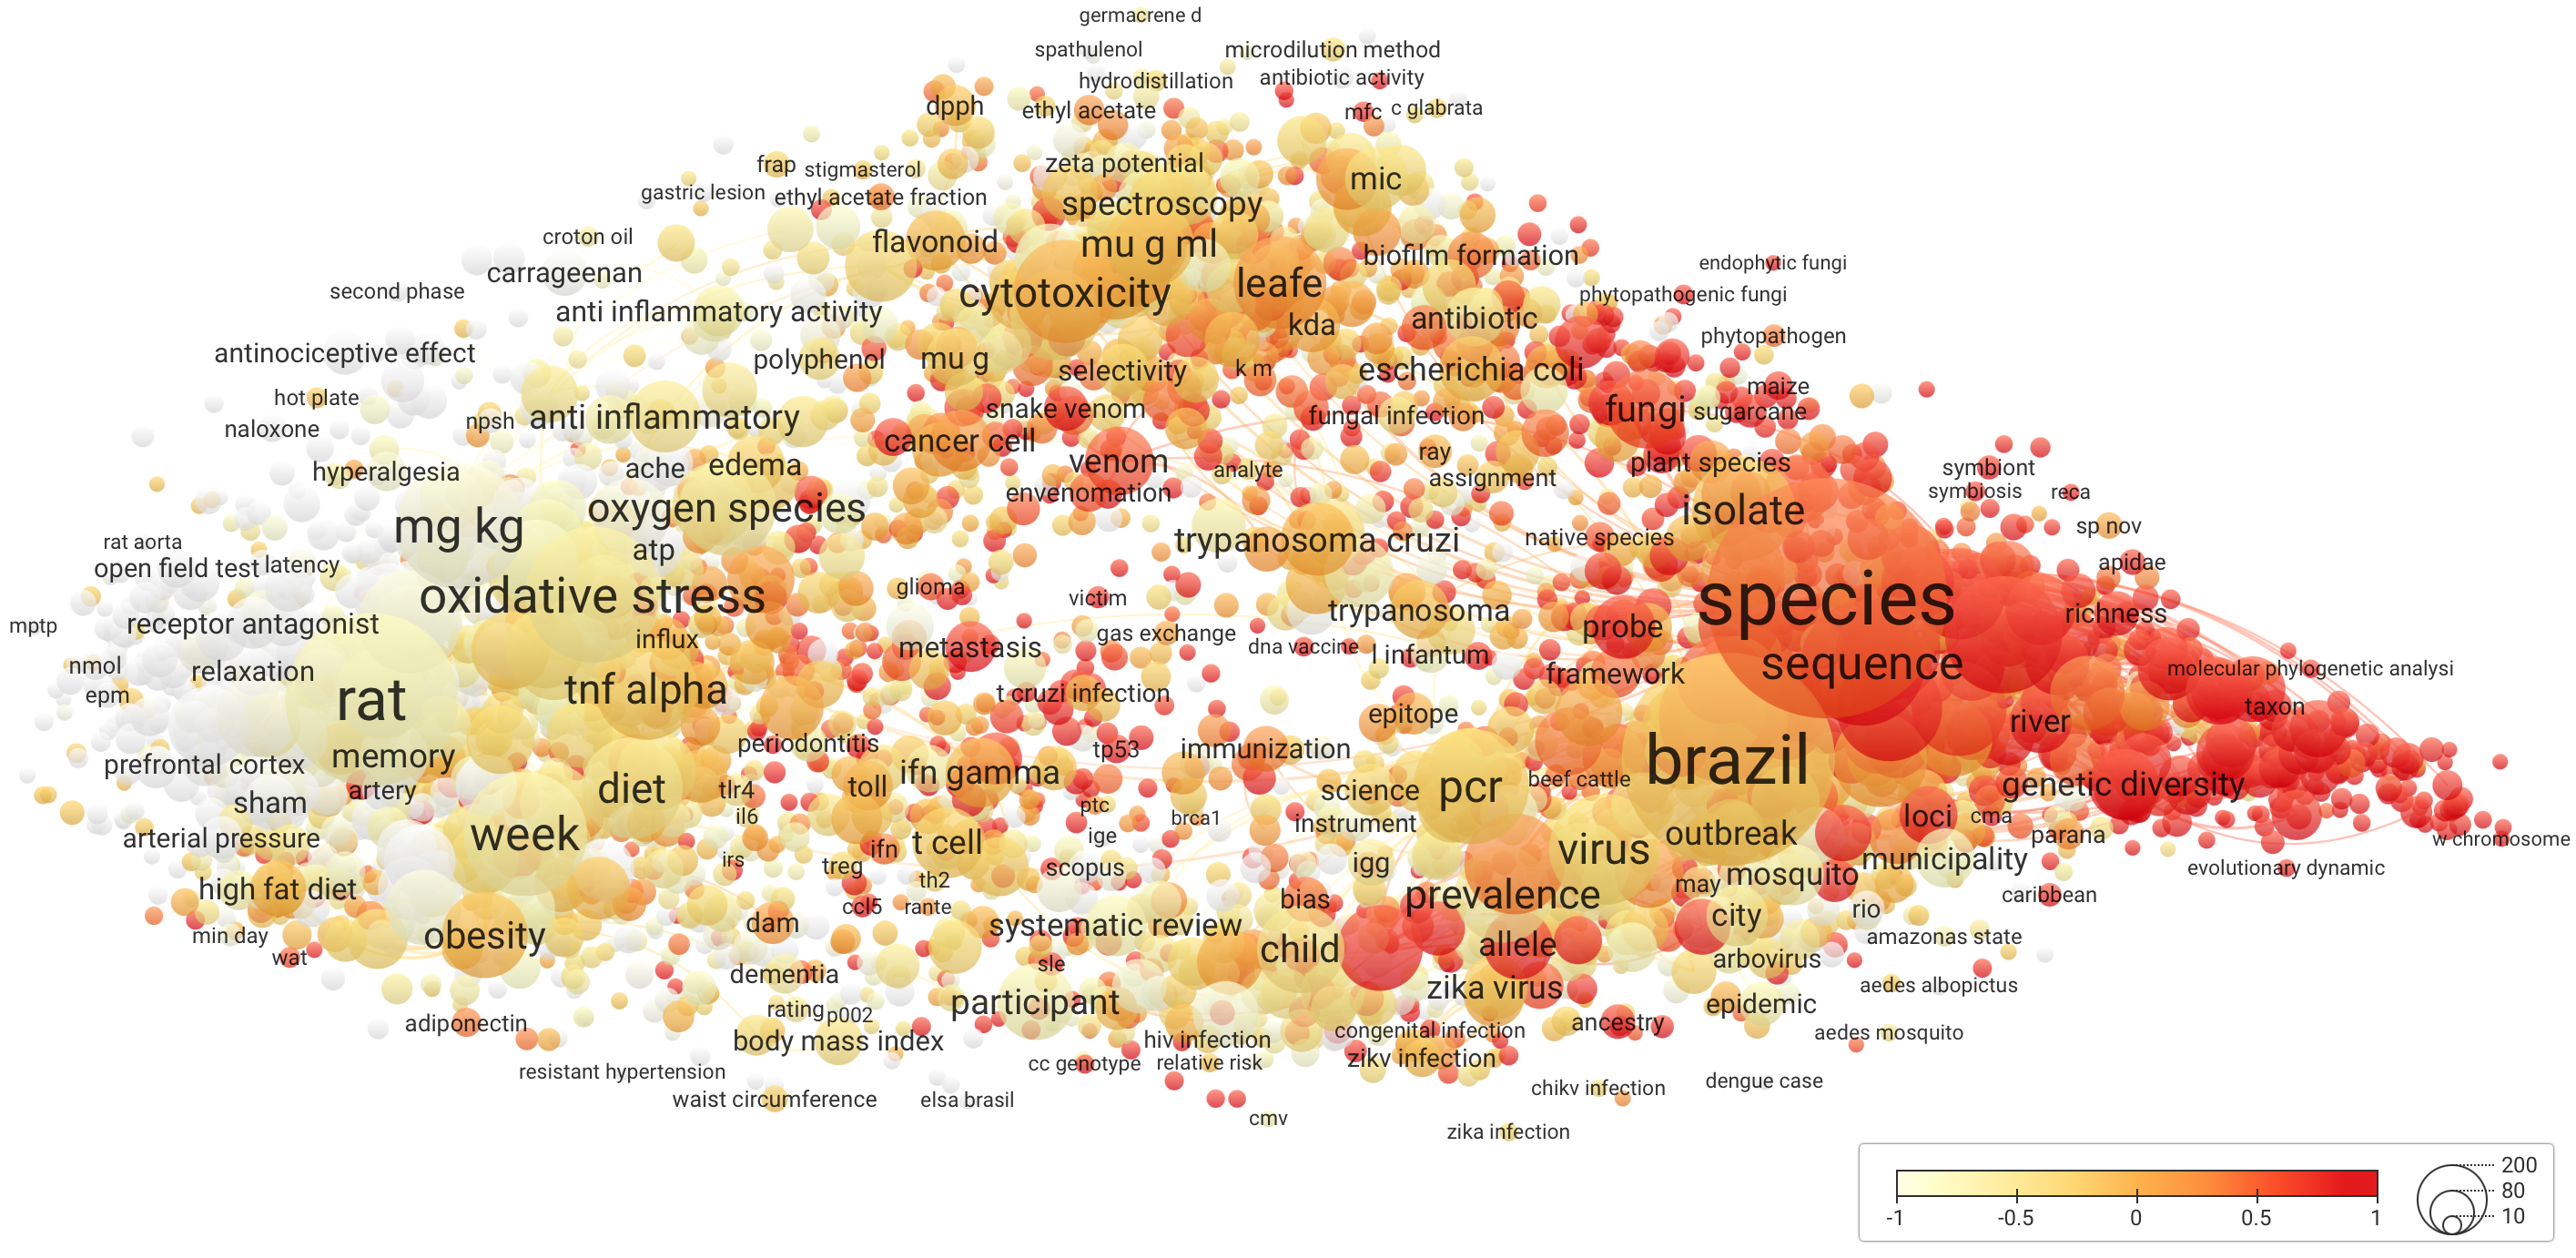
\includegraphics[width=1\textwidth]{images/chapter_classific/VOSviewer-CBI.png}\label{fig:classif:vosviewer_cb1}
    \vspace{-20em}\caption{Biological Sciences I}
  \end{subfigure}
  \\
  \begin{subfigure}[t]{1\textwidth}
     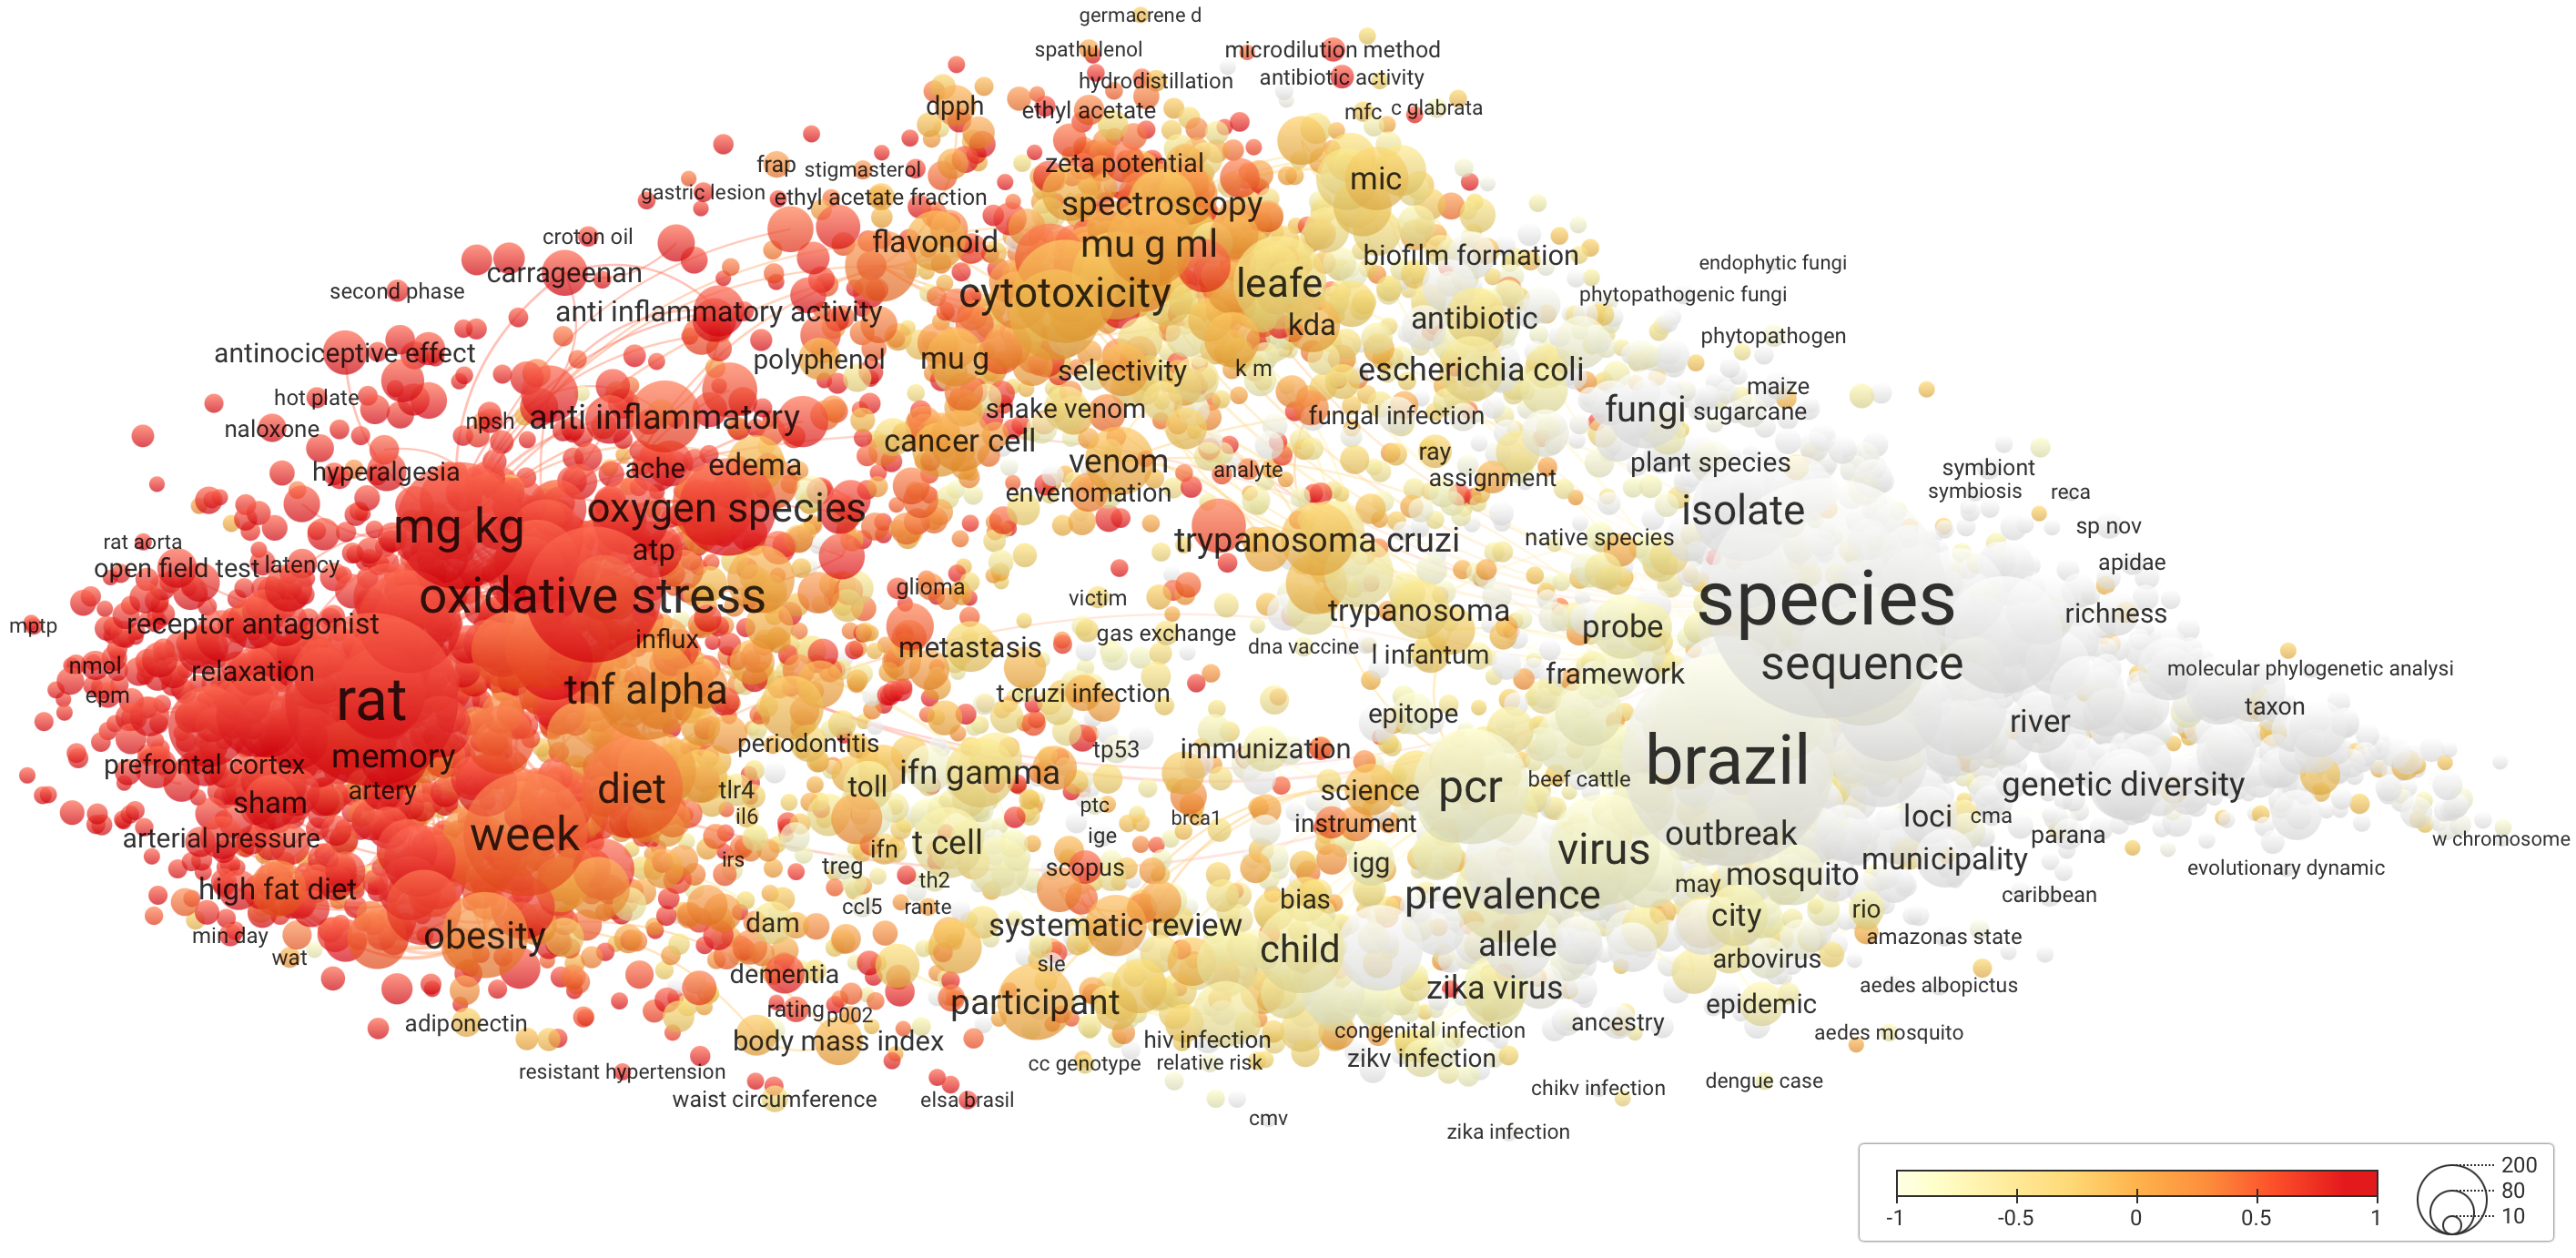
\includegraphics[width=1\textwidth]{images/chapter_classific/VOSviewer-CBII.png}\label{fig:classif:vosviewer_cb2}
    \vspace{-20em}\caption{Biological Sciences II}
  \end{subfigure}
  \\
  \begin{subfigure}[t]{1\textwidth}
     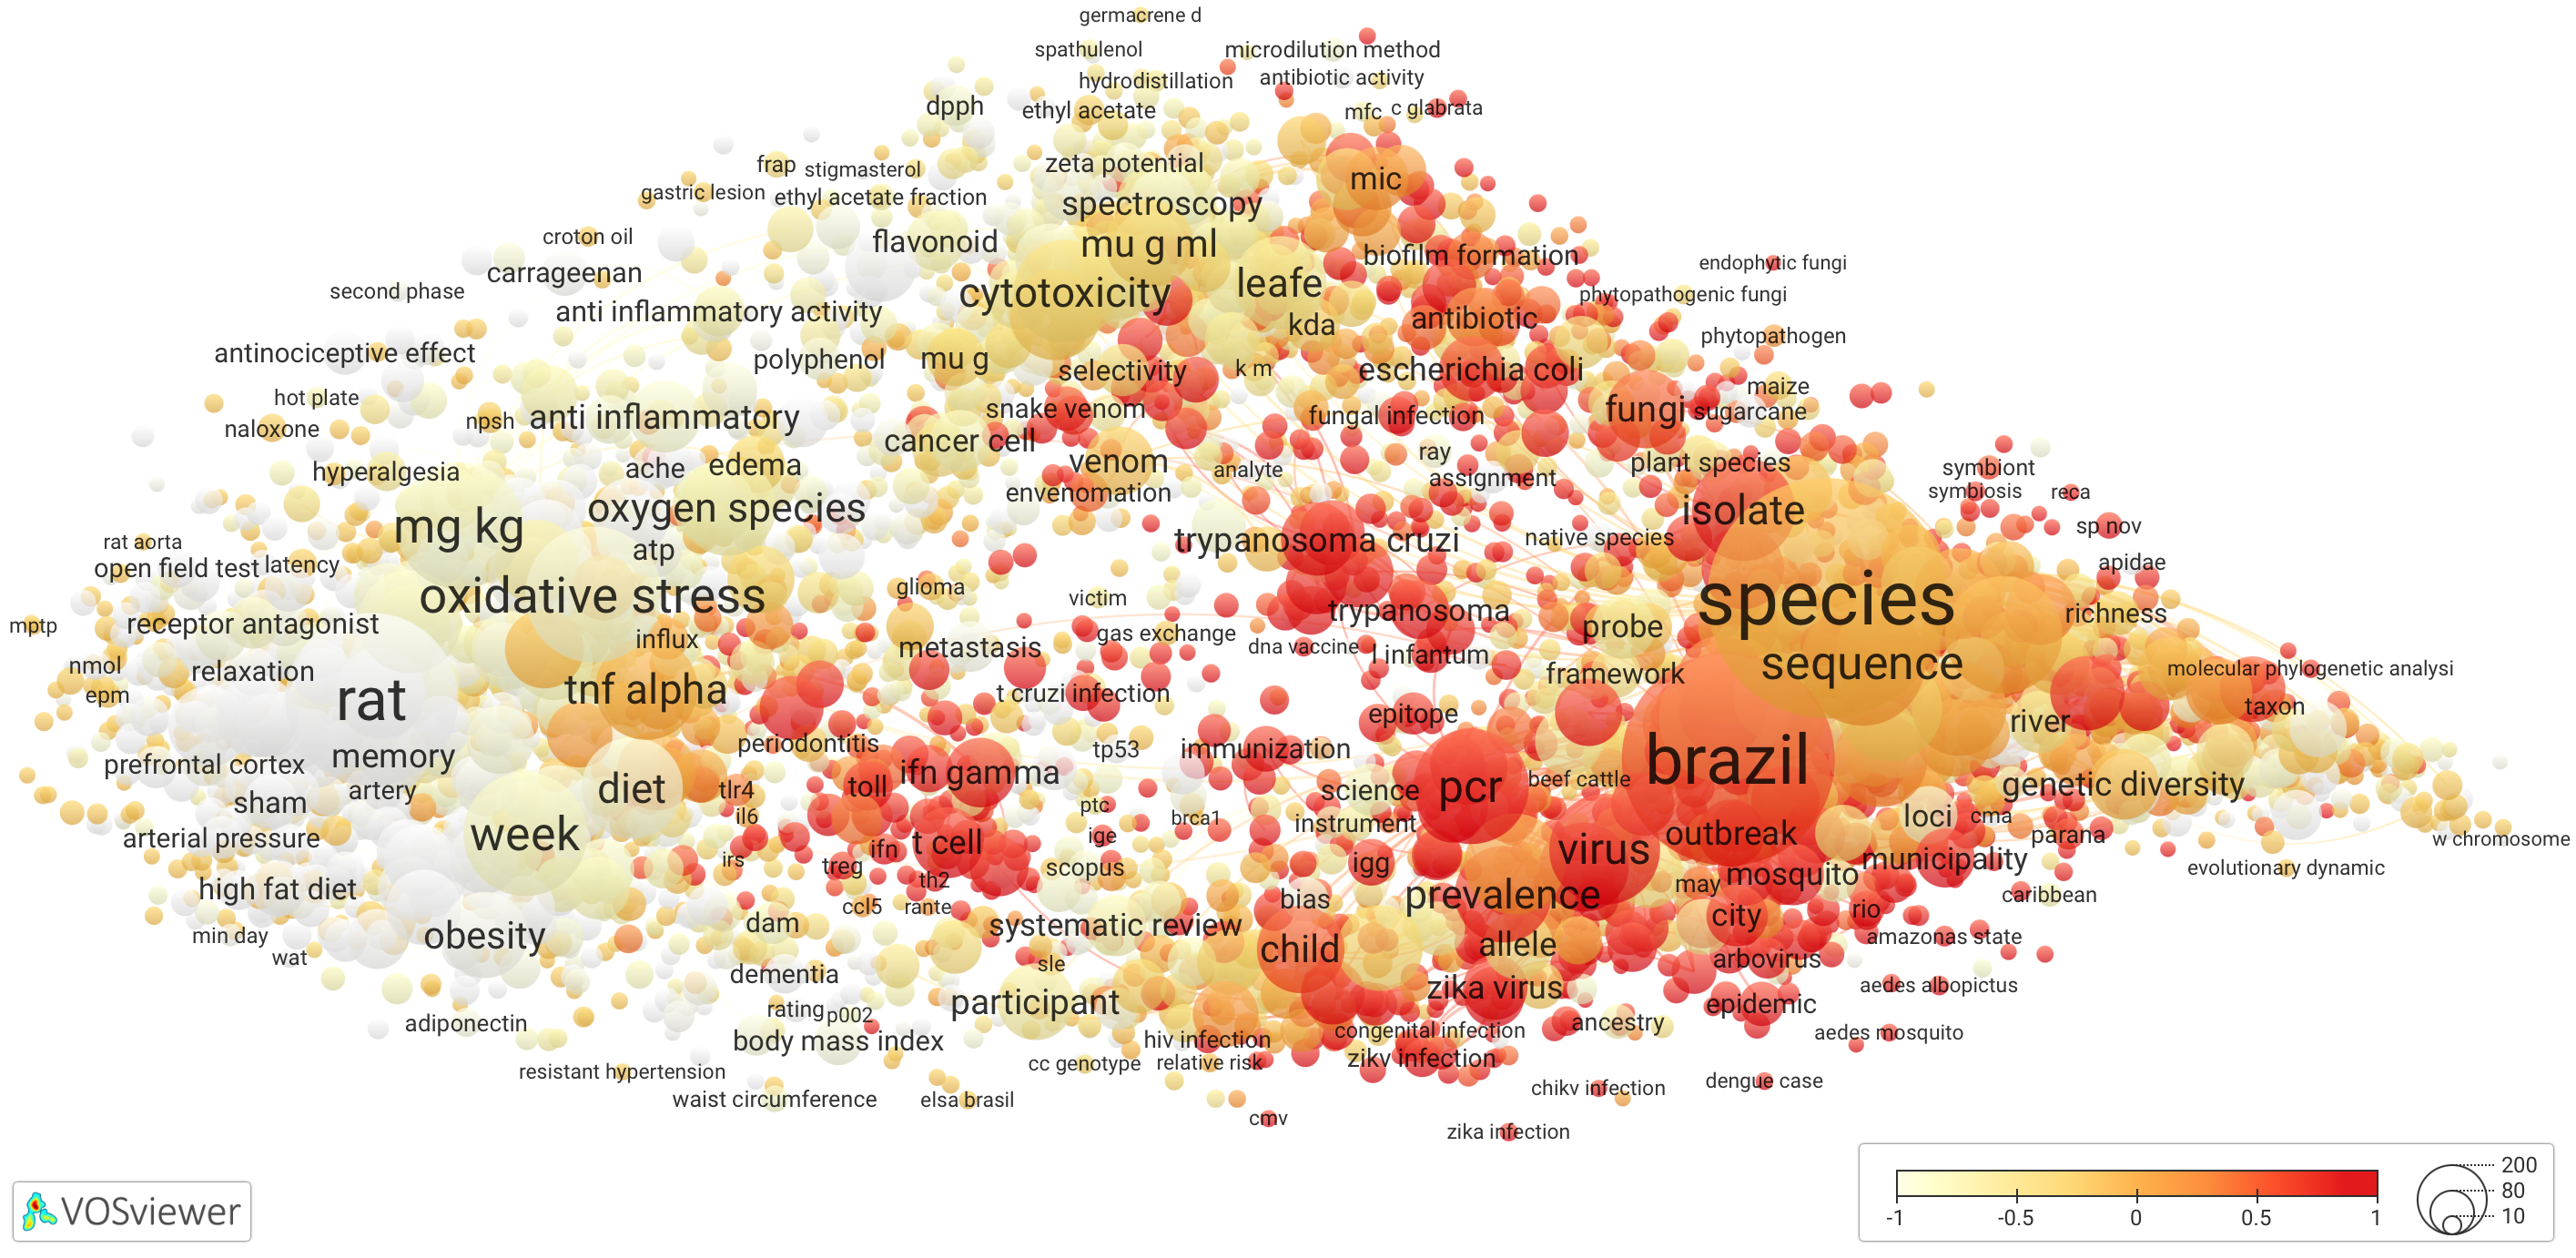
\includegraphics[width=1\textwidth]{images/chapter_classific/VOSviewer-CBIII.png}\label{fig:classif:vosviewer_cb3}
    \vspace{-20em}\caption{Biological Sciences III}
  \end{subfigure}
    \caption{Term maps of papers from the BioSci evaluation areas, with a colour overlay highlighting publications of each area (2017-2018)}
    \label{fig:classif:vosviewer_cb_all}
\end{figure}
 
The bibliometric profiles in \Cref{fig:classif:vosviewer_cb_all} are revealing. First, we notice that BioSci I (\subref{fig:classif:vosviewer_cb1}) and II (\subref{fig:classif:vosviewer_cb2}) operate on opposite sides of the term map, revealing the areas focus most of their attention on specific research interests. Regarding BioSci III (\subref{fig:classif:vosviewer_cb3}), the area operates toward the middle of the map, slightly overlapping BioSci I, but with increased attention to issues such as parasitology and immunology, and with added focus on issues of regional interest (observed in the ‘Brazil’ cluster). Although an expert committee could reach more robust conclusions from the provided maps, deciding whether the three areas need adjustment, the bibliometric perspective indicates that the research outputs of each area align with their associated subareas and specialties listed in CAPES’ classification document \autocite*{CAPES.2020tb}.

Another application of term maps, as seen in \Cref{fig:classif:vosviewer_cb_ppg}, is to focus on the profiles of individual graduate programs and how their research compares with the broader map of BioSci research. 

\begin{figure}[H]
\vspace{12pt}
\captionsetup[sub]{justification=raggedright, singlelinecheck=false}
  \begin{subfigure}[t]{.48\textwidth}
    \centering
    \caption{PPG 32001010175P5 – BioSci I}
    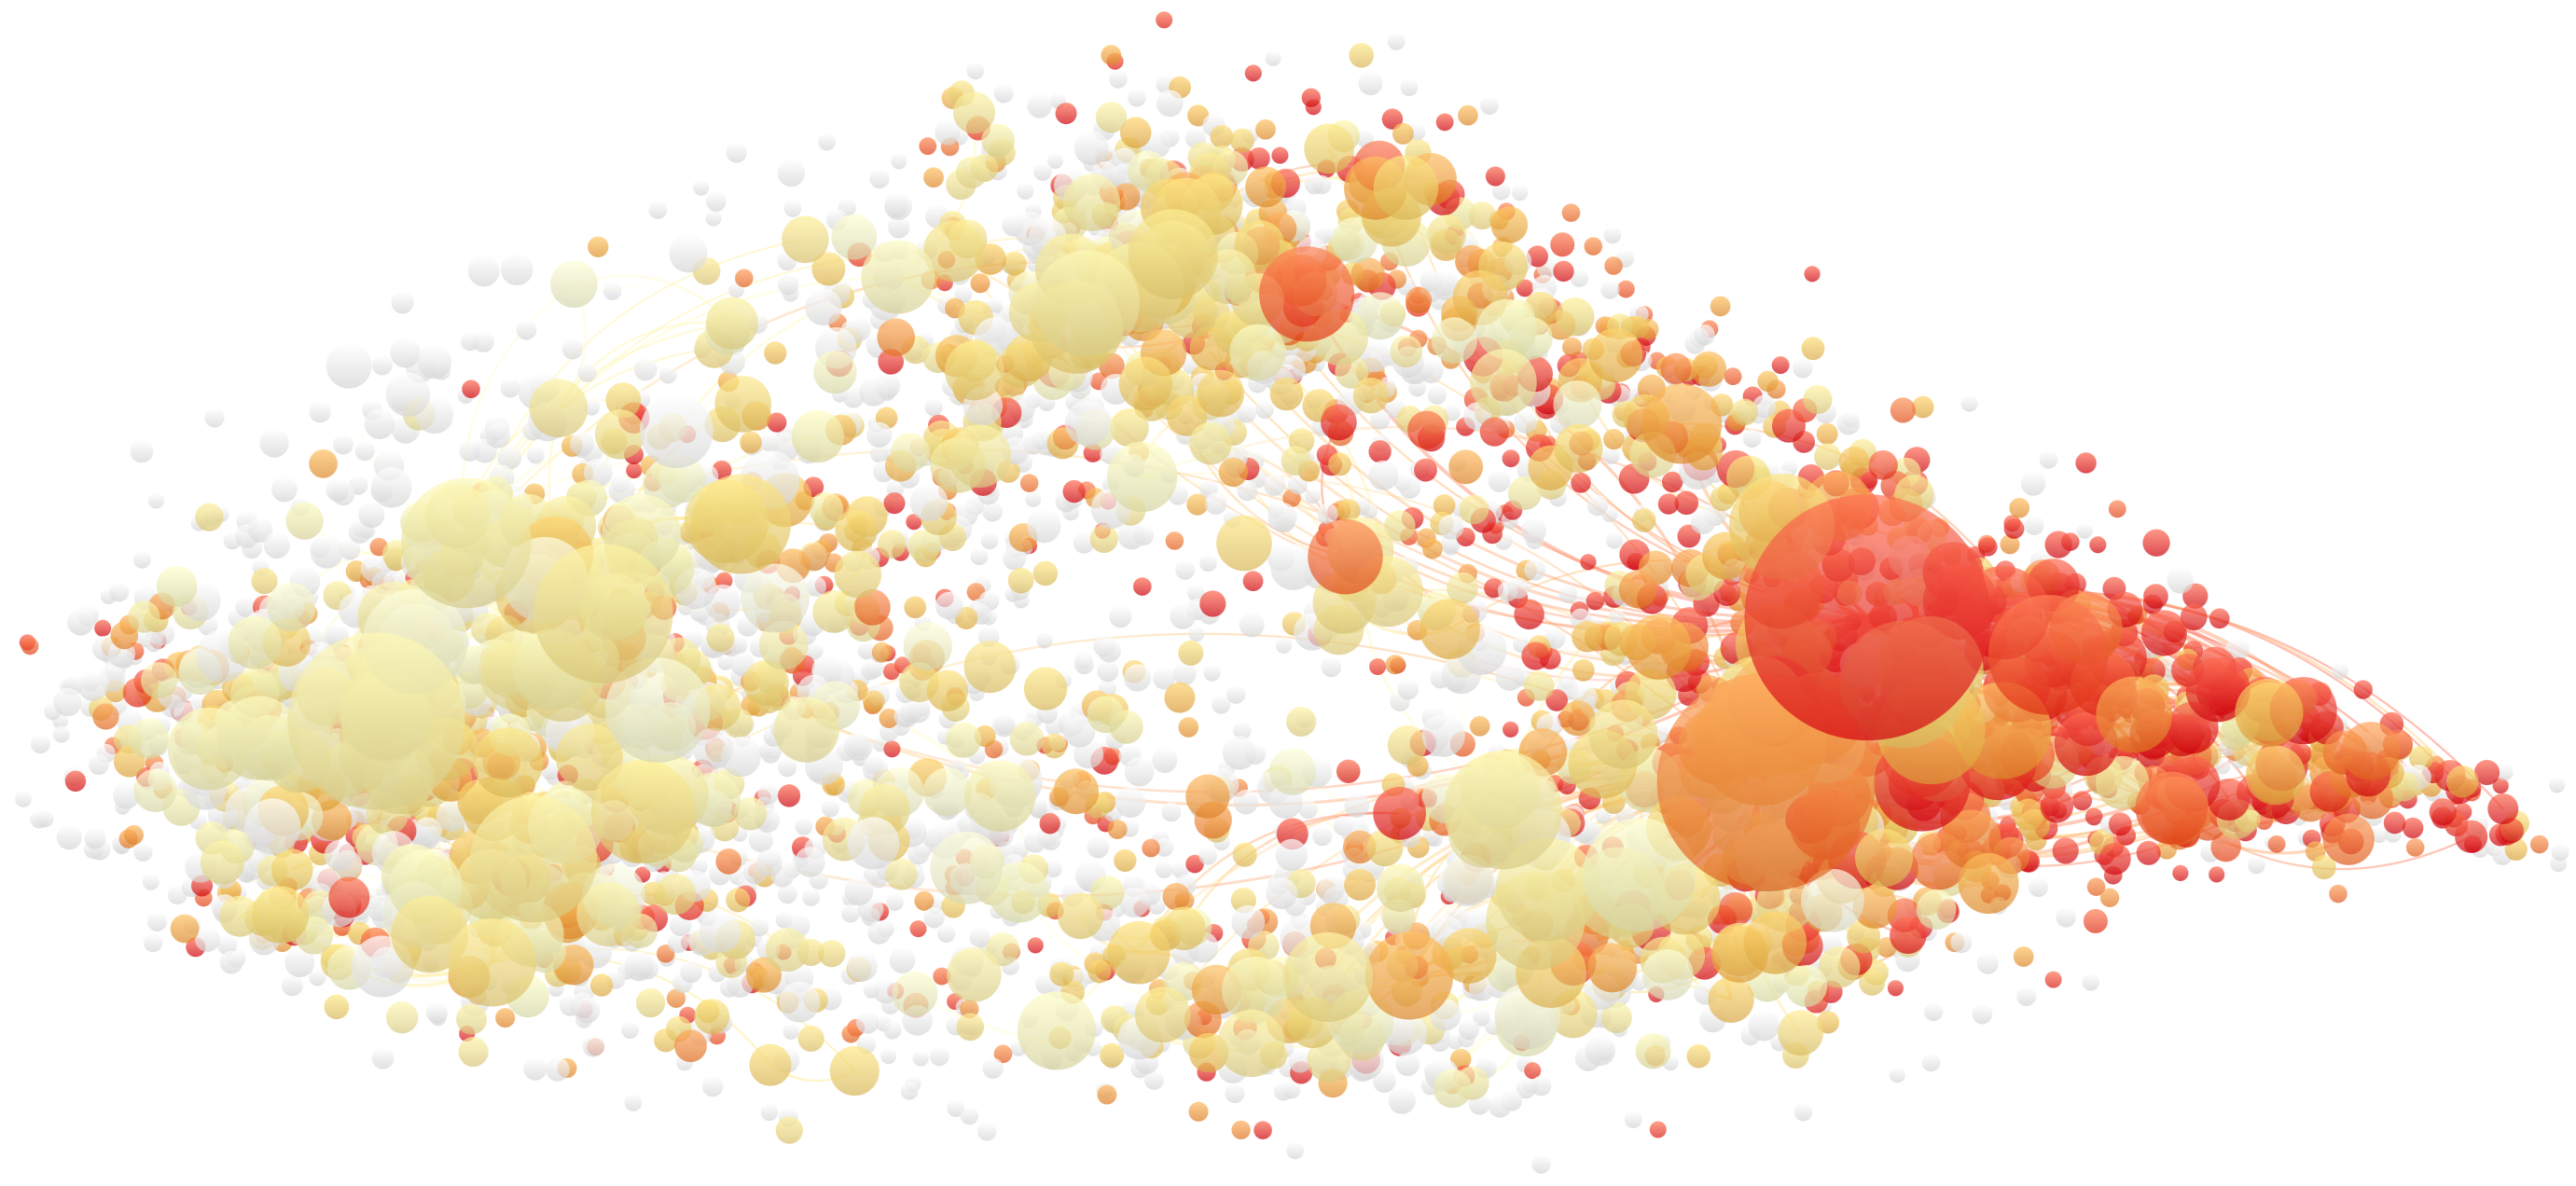
\includegraphics[width=\linewidth]{images/chapter_classific/VOSviewer-CBIa.png}
    \label{fig:classif:vosviewer_cb1a}
  \end{subfigure}
  \hfill
  \begin{subfigure}[t]{.48\textwidth}
    \centering
    \caption{PPG 32001010068P4 – BioSci I}
    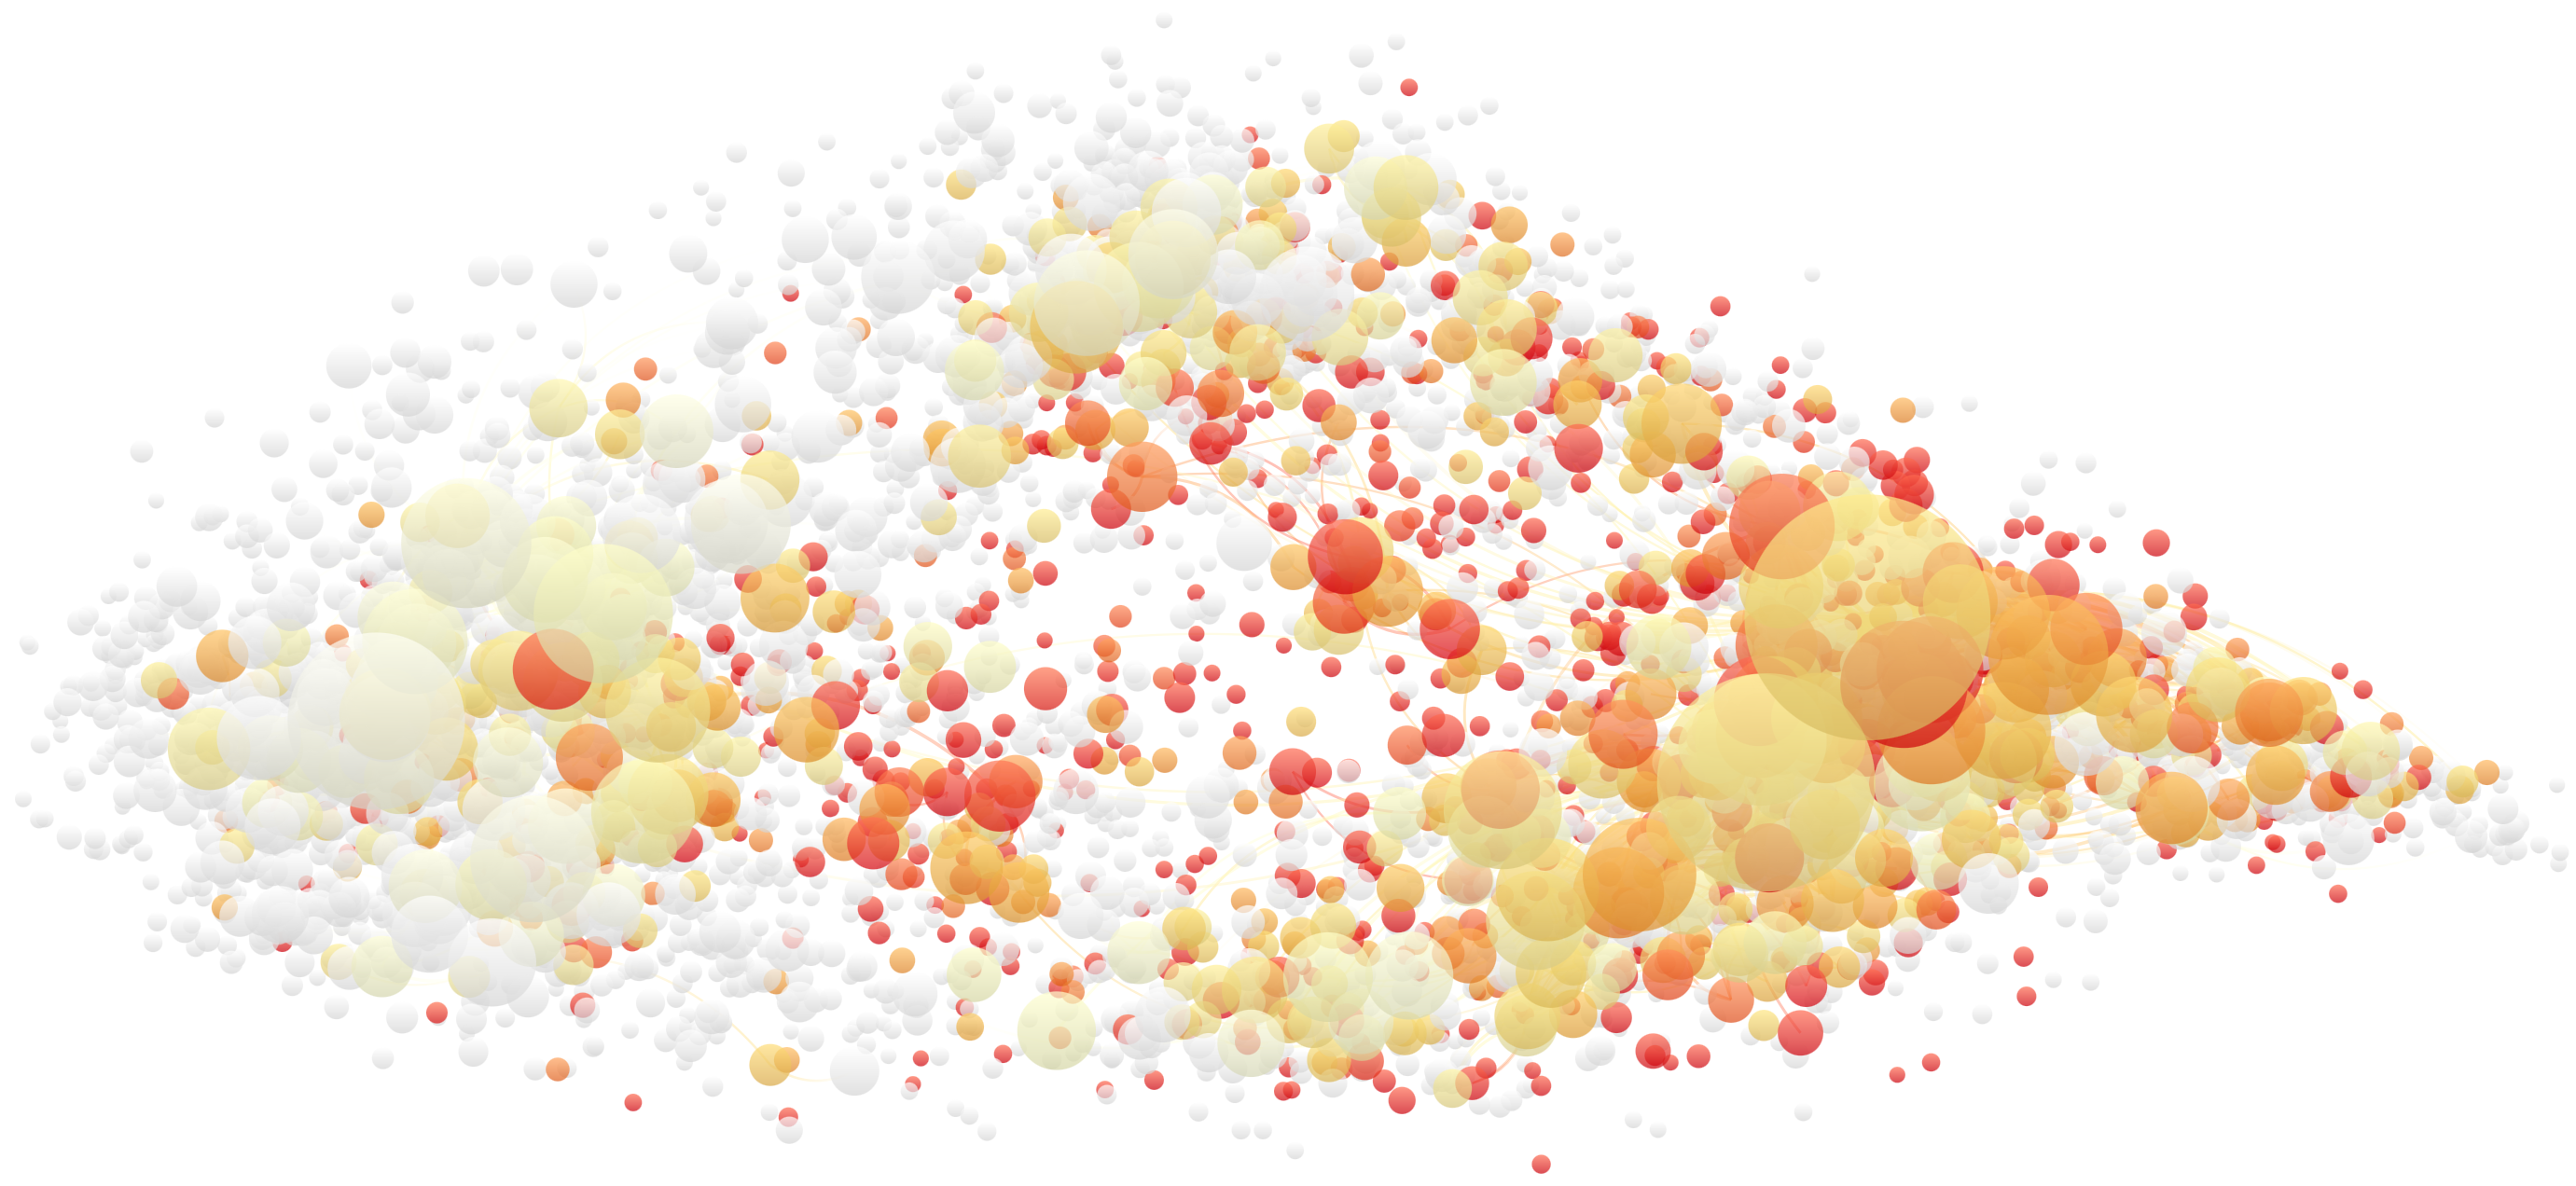
\includegraphics[width=\linewidth]{images/chapter_classific/VOSviewer-CBIb.png}
    \label{fig:classif:vosviewer_cb1b}
  \end{subfigure}\\ %\vspace{-0.6em}
    \begin{subfigure}[t]{.48\textwidth}
    \centering
    \caption{PPG 42002010023P9 – BioSci II}
    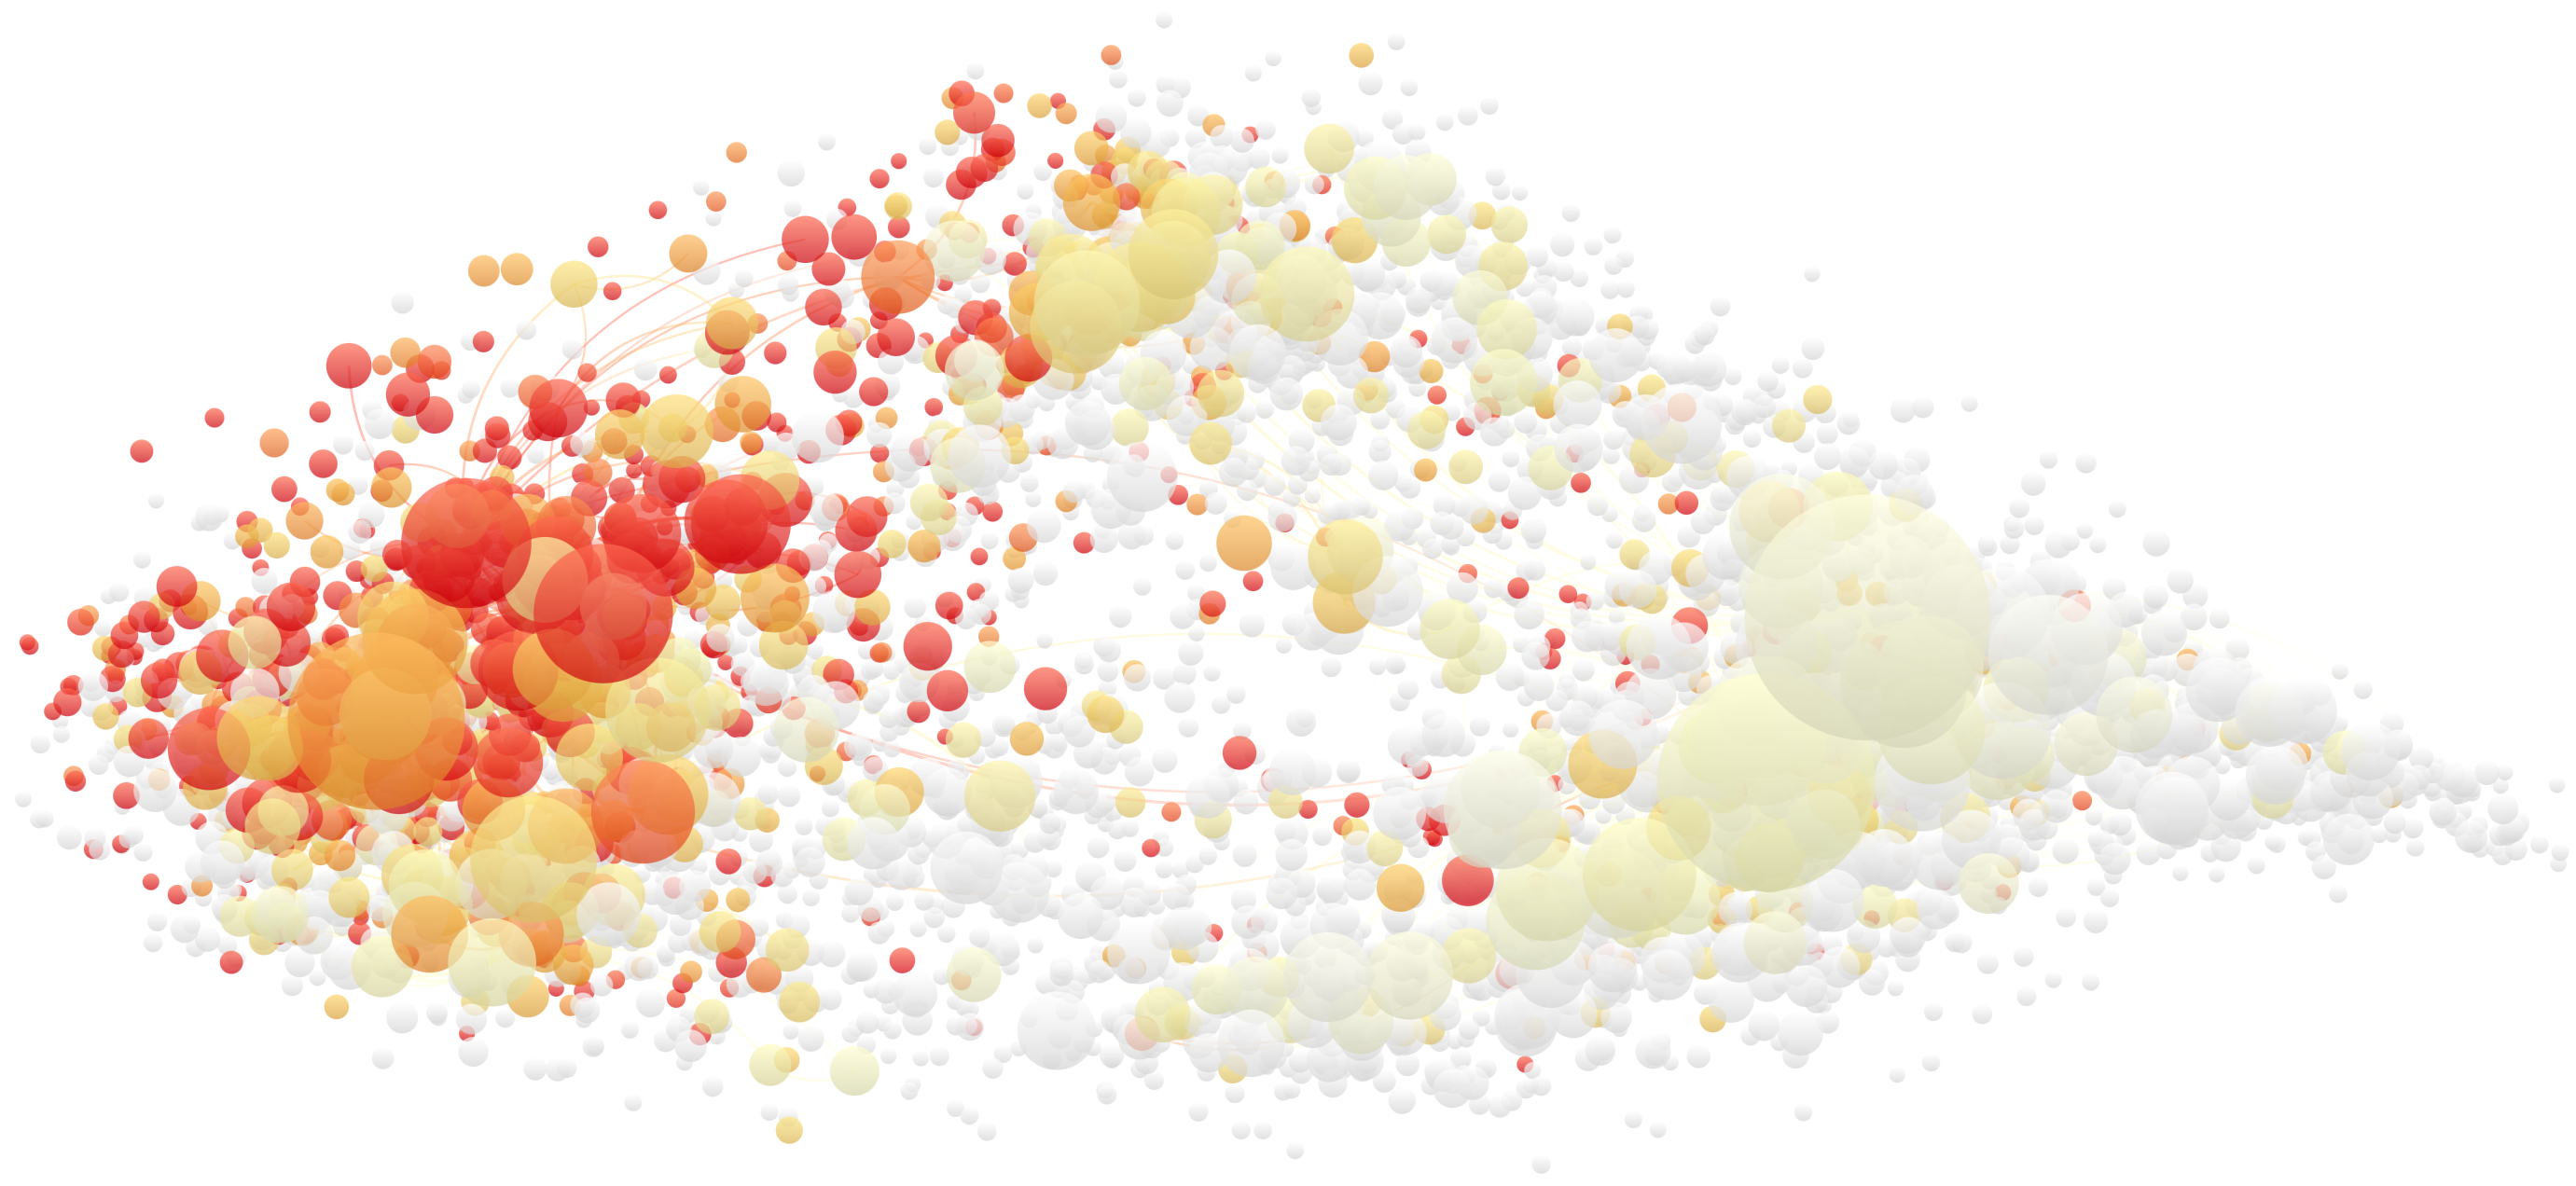
\includegraphics[width=\linewidth]{images/chapter_classific/VOSviewer-CBIIa.png}
    \label{fig:classif:vosviewer_cb2a}
  \end{subfigure}
  \hfill
  \begin{subfigure}[t]{.48\textwidth}
    \centering
    \caption{PPG 31010016004P9 – BioSci II}
    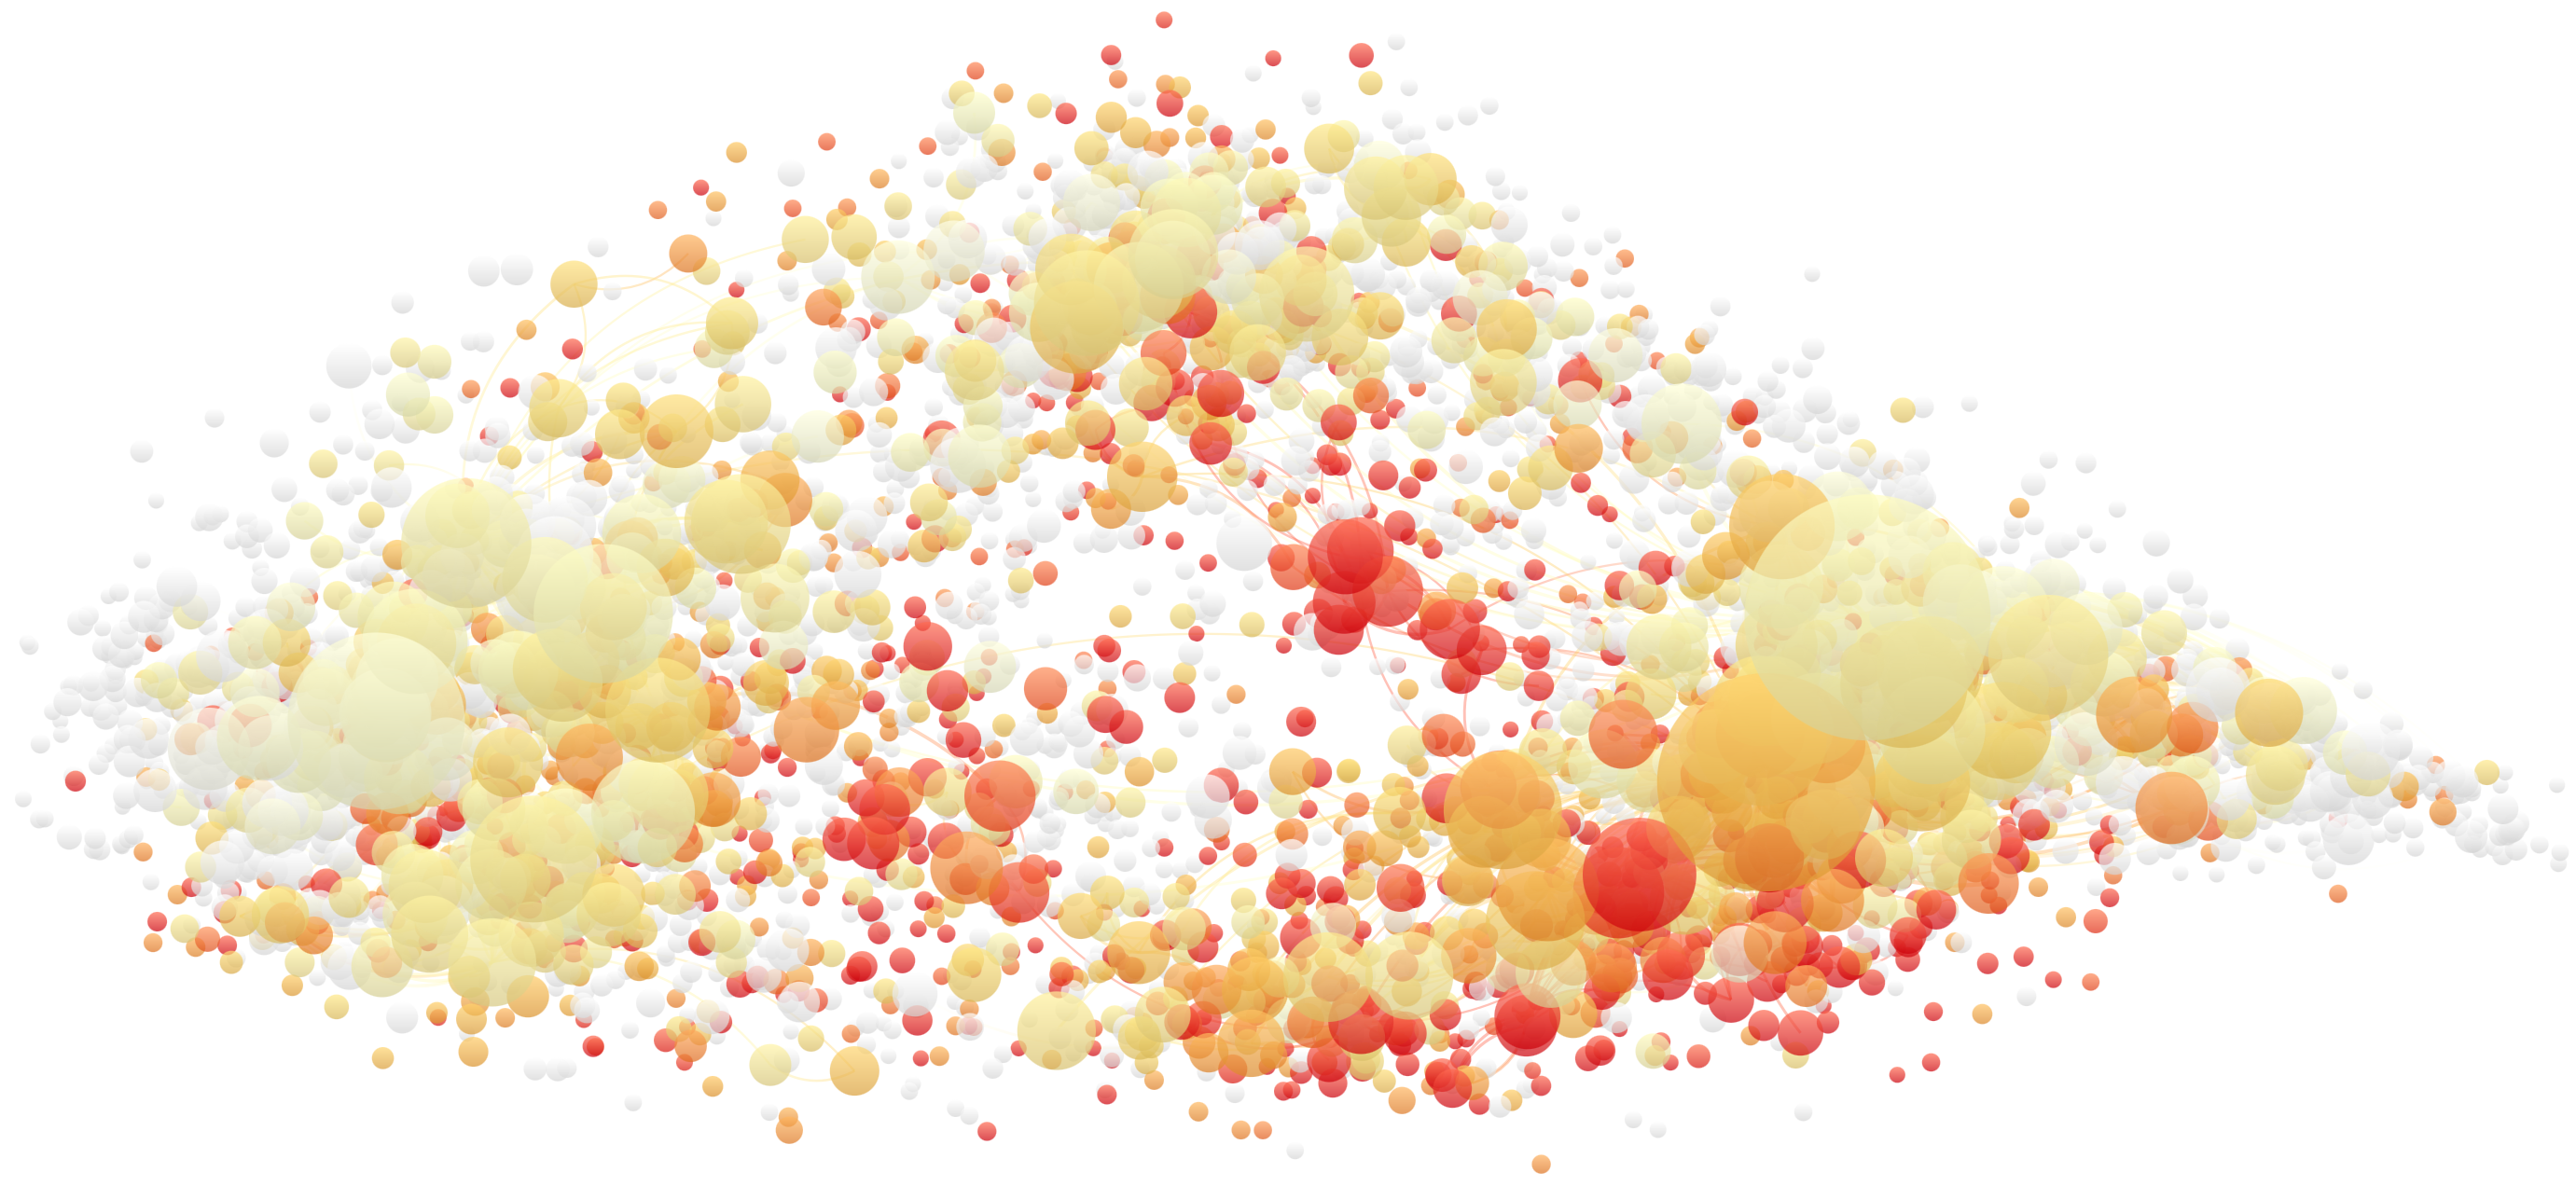
\includegraphics[width=\linewidth]{images/chapter_classific/VOSviewer-CBIIb.png}
    \label{fig:classif:vosviewer_cb2b}
  \end{subfigure}\\ %\vspace{-0.6em}
    \begin{subfigure}[t]{.48\textwidth}
    \centering
    \caption{PPG 33002010022P3 – BioSci III}
    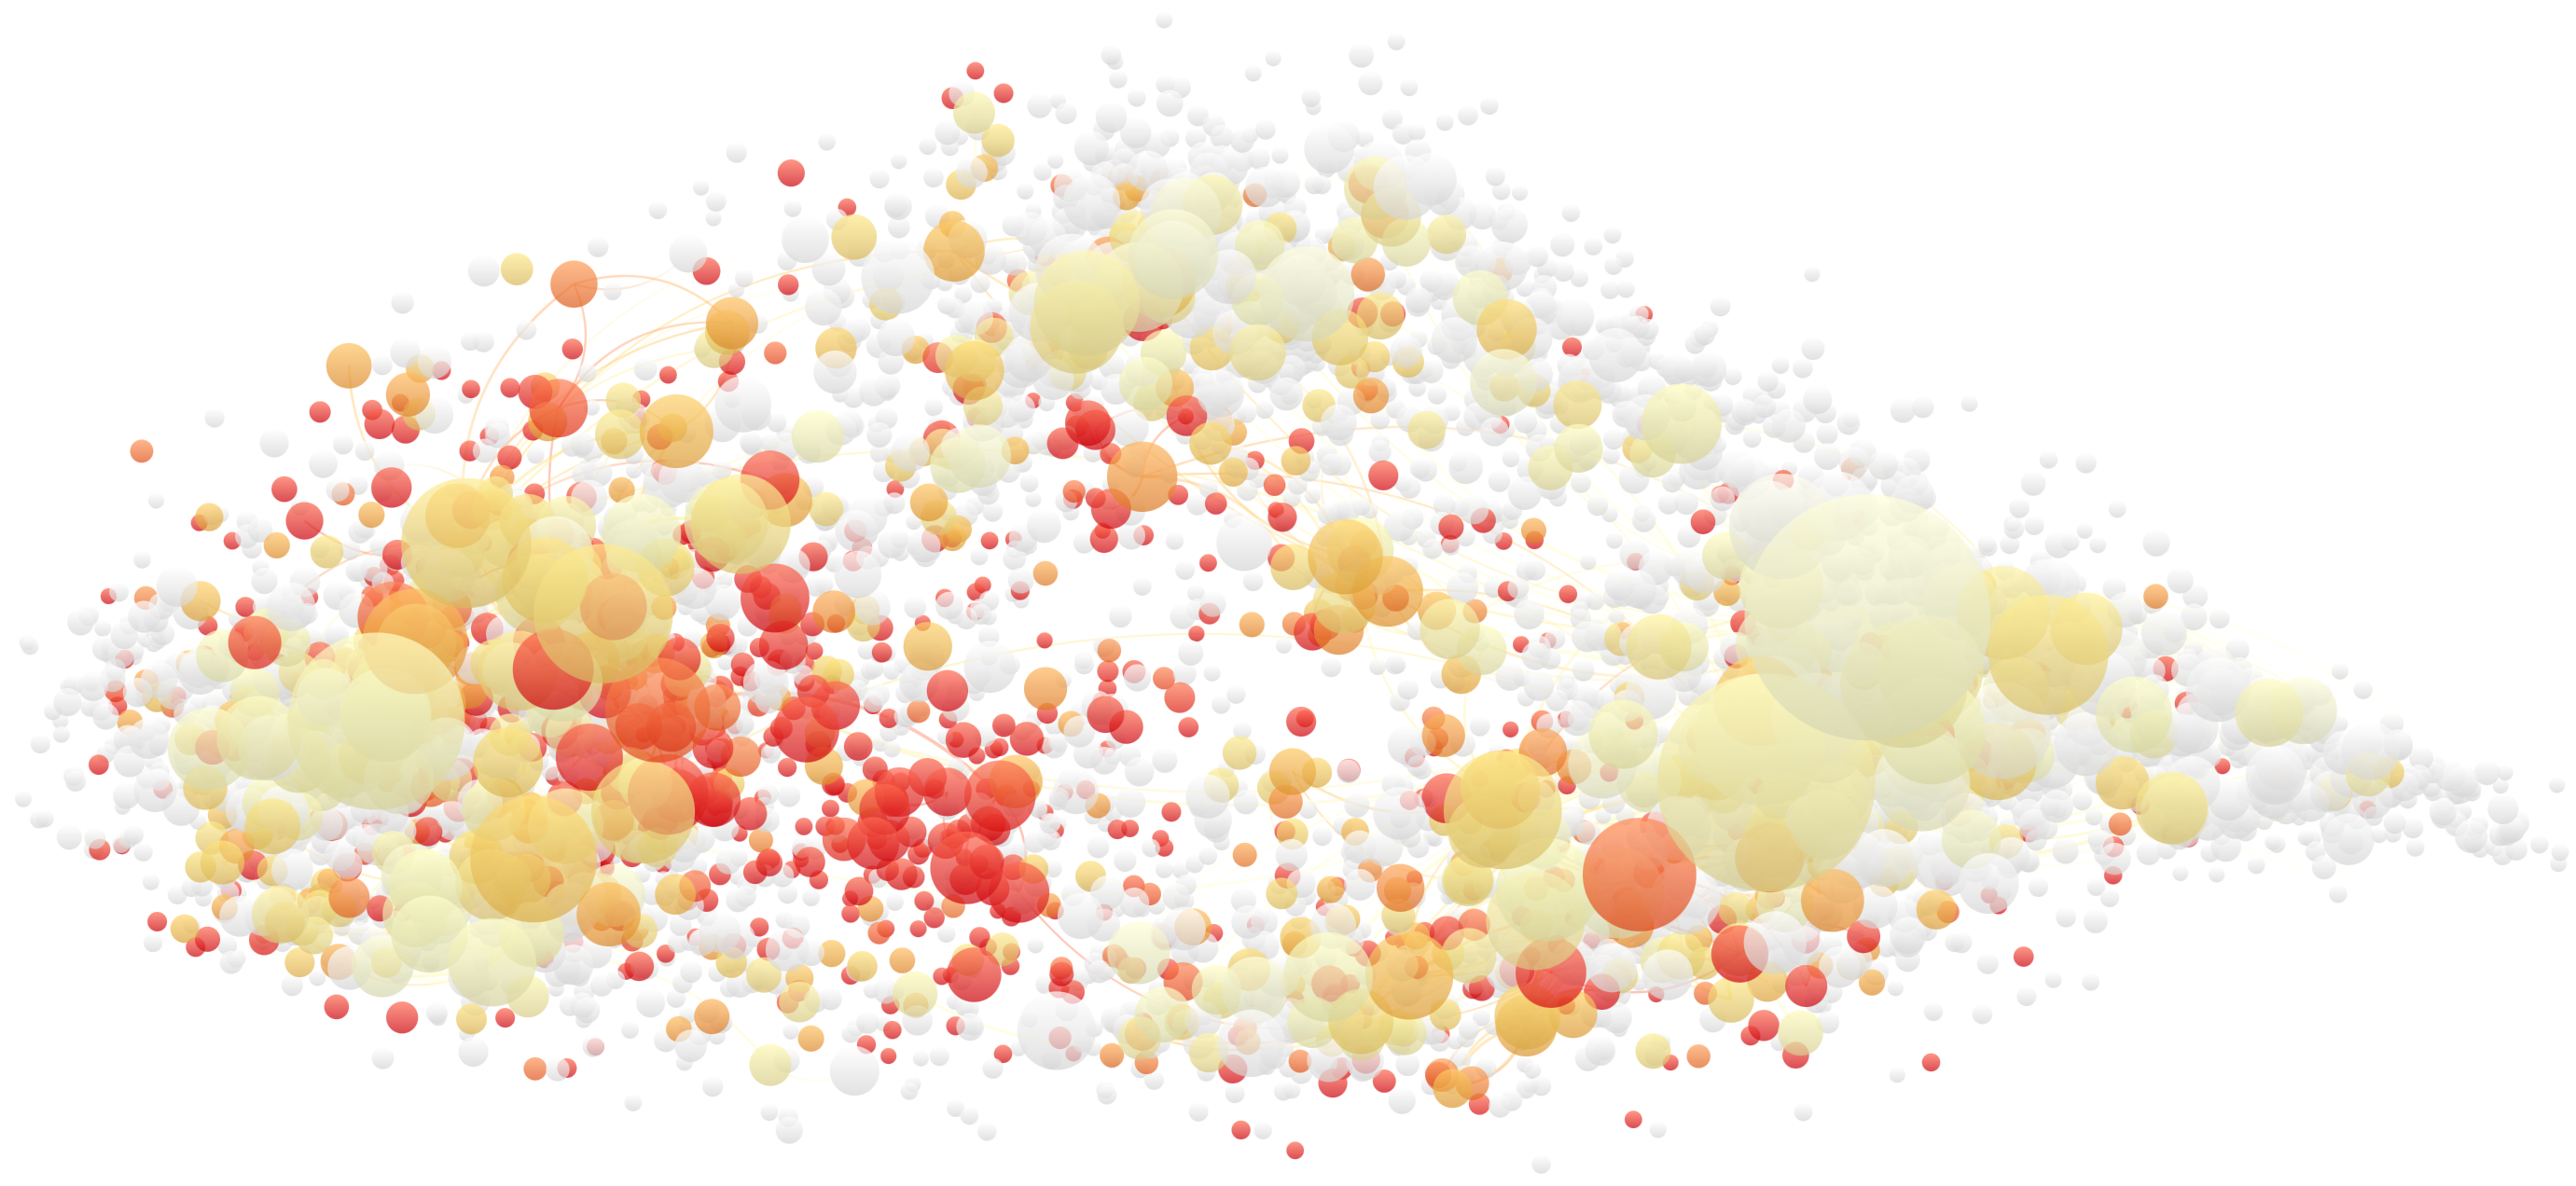
\includegraphics[width=\linewidth]{images/chapter_classific/VOSviewer-CBIIIa.png}
    \label{fig:classif:vosviewer_cb3a}
  \end{subfigure}
  \hfill
  \begin{subfigure}[t]{.48\textwidth}
    \centering
    \caption{PPG 33002029026P4 – BioSci III}
    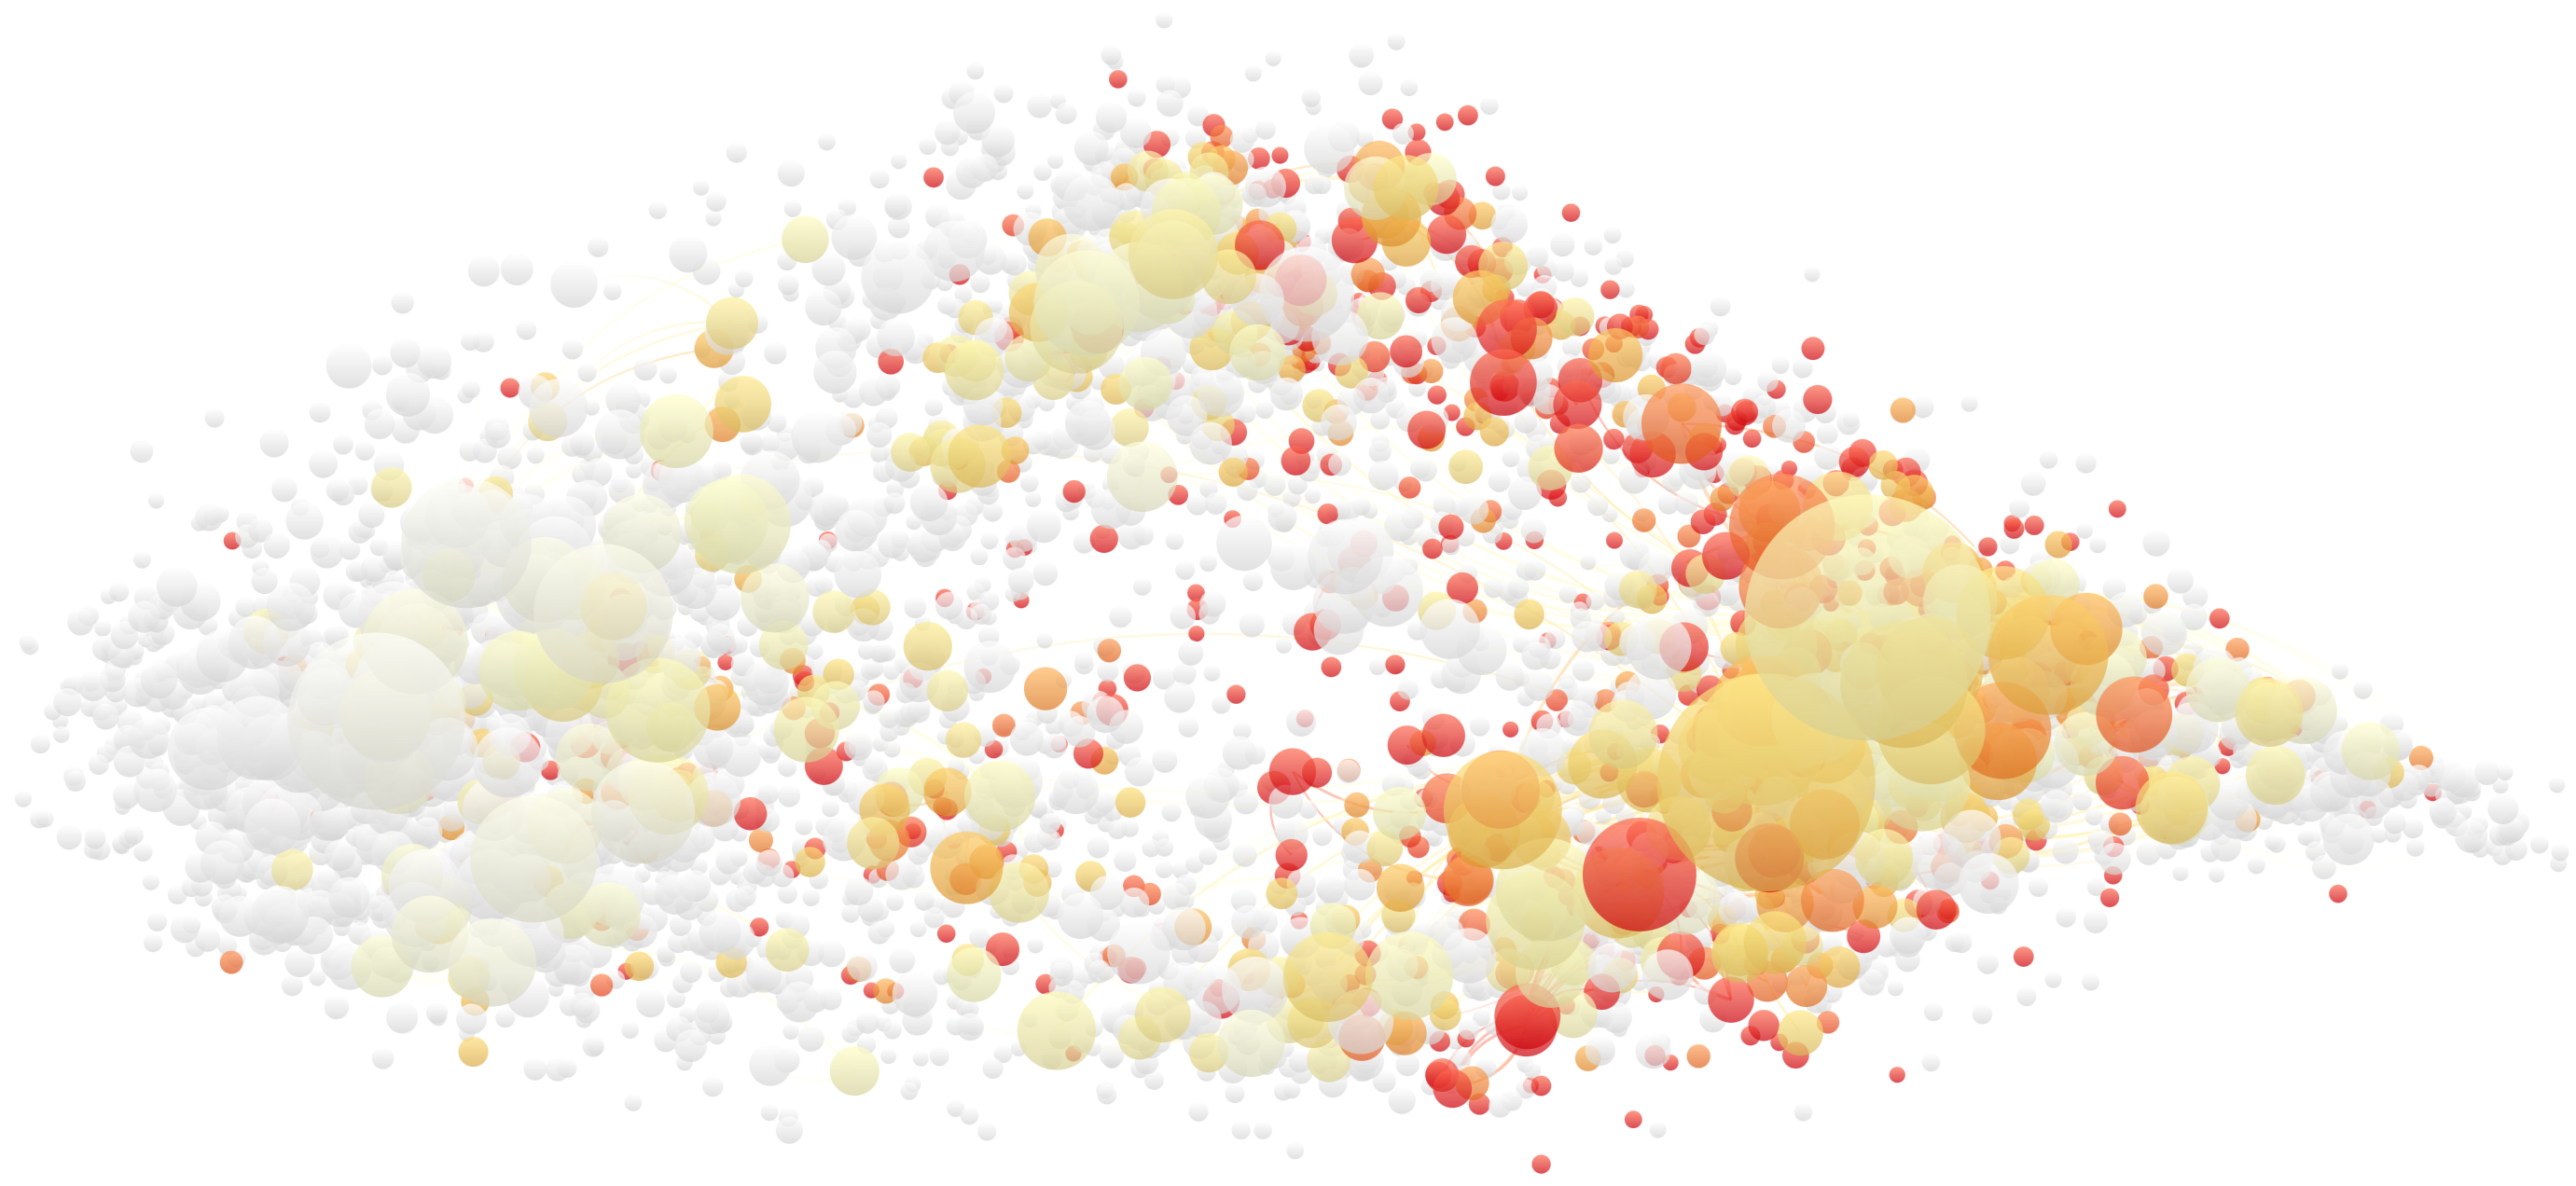
\includegraphics[width=\linewidth]{images/chapter_classific/VOSviewer-CBIIIb.png}
    \label{fig:classif:vosviewer_cb3b}
  \end{subfigure}\\ %\vspace{-0.6em}
  \centering 
    \caption{Term maps of papers from the BioSci evaluation areas, highlighting the publication profiles of individual PPG (2017-2018).}
\label{fig:classif:vosviewer_cb_ppg}
\end{figure} 	 

\Cref{fig:classif:vosviewer_cb_ppg} shows publication profiles of two graduate programs in each BioSci. The term maps shown on the left (\subref{fig:classif:vosviewer_cb1a}, \subref{fig:classif:vosviewer_cb2a}, and \subref{fig:classif:vosviewer_cb3a}) are from graduate programs whose profiles fit within the publication topics shown in \Cref{fig:classif:vosviewer_cb_ppg} for their respective areas. However, the maps shown on the right (\subref{fig:classif:vosviewer_cb1b}, \subref{fig:classif:vosviewer_cb2b}, and \subref{fig:classif:vosviewer_cb3b}) are examples of PPG profiles that may be more well-suited with different evaluation areas, suggesting that some programs associated with the current BioSci areas may need to migrate. Once again, that analysis can only be performed by experts in the respective disciplines, but the proposed approach seems to be a promising way to aid them in such a task.

\section{Conclusions}
\label{sec:classif:Conclusions}

This study investigated the Brazilian classification system for research and graduate education. The motivations behind the system design were examined, as well as some central factors in its evolution and expansion. From this, it was possible to identify that the current system became somewhat peculiar in its distinctions from international classification systems such as OECD’s Fields of Research and Development (FORD) and the International Standard Classification of Education (ISCED). In particular, the misalignment among the evaluation and broad areas of the Brazilian system and their corresponding levels in the analysed alternatives is significant, especially in the SSH profiles.

From the differences mapped in this study, it became evident that the Brazilian system needs revision, an idea aligned with recommendations from the special committee in charge of monitoring the Brazilian National Plan for Research and Graduate Education. Although the \textcite{CEPNPG.2020} suggested a significant reduction in the number of evaluation areas, this study proposes adopting bibliometrics to delineate new areas based on the affinity of the research conducted within graduate programs, the central unit of the research system in Brazil.

Due to the limitations of a short paper format, this study focused on presenting a potential method based on term maps capable of highlighting publication profiles from both evaluation areas and graduate programs. The results seem robust enough to be useful in aiding expert committees to restructure the Brazilian classification system. An additional approach would count with the application of the Leiden Algorithm \autocite{Traag.2019} to analyse citation relations connecting research results from the Brazilian science system. Such an approach, which will be presented in an upcoming extended version of this paper, can complement the resources informing a review of the classification that is based on evidence and not on any simplistic approach.